\documentclass[pdflatex,sn-mathphys]{sn-jnl} % Springer Nature template for NCA

%------------------------------------------------------------------------------
% PACKAGES
%---------------------------------------------------------------------------

\usepackage[normalem]{ulem}

\usepackage{amsmath,amssymb,amsfonts}
\usepackage{graphicx}
\graphicspath{{figures/}}
\usepackage{booktabs}
\usepackage{array}
\usepackage{float}
\usepackage{flafter} % a float never appears before its first reference
% Keep floats close to where they are introduced
\renewcommand{\topfraction}{0.9}
\renewcommand{\bottomfraction}{0.8}
\renewcommand{\textfraction}{0.07}
\renewcommand{\floatpagefraction}{0.7}
\setcounter{topnumber}{4}
\setcounter{bottomnumber}{3}
\setcounter{totalnumber}{6}
\usepackage{subcaption}
\usepackage{caption}
\usepackage[table]{xcolor}
\usepackage{hyperref}
\hypersetup{colorlinks=true, allcolors=blue}
\usepackage{textcomp}
\usepackage[numbers]{natbib}
\usepackage{rotating}
\raggedbottom

%------------------------------------------------------------------------------
% BEGIN DOCUMENT
%------------------------------------------------------------------------------
\begin{document}

%------------------------------------------------------------------------------
% TITLE AND AUTHORS
%------------------------------------------------------------------------------
\title[Spatial Transfer in Crop Classification]{Spatial Transfer Reorders Crop Classifiers --- and Sparse Feature Selection Explains Why: A Multi-Model Benchmark on Sentinel-2 Time Series}
\makeatletter
\renewcommand{\@makefnmark}{\textsuperscript{*}}
\renewcommand{\footnoterule}{
  \kern -3pt
  \hrule width 2cm height 0.4pt
  \kern 2.6pt
}
\makeatother
\footnotetext{Corresponding author: Disha Kacha, disha.kacha@gwu.edu}
\author[2]{\fnm{Michael} \sur{Mann}}\email{mmann1123@email.gwu.edu}
\author[1]{\fnm{Sairam} \sur{Venkatachalam}}\email{sairam.venkatachalam@gwu.edu}
\author[1]{\fnm{Disha} \sur{Kacha}}\email{disha.kacha@gwu.edu}
\author[1]{\fnm{Devarsh} \sur{Sheth}}\email{devarshapurva.sheth@gwu.edu}
\author[2]{\fnm{Amir} \sur{Jafari}}\email{ajafari@email.gwu.edu}

\affil{\orgdiv{Department of Geography \& Environment and the Data Science Program}, \orgname{The George Washington University}, \city{Washington}, \state{DC}, \country{USA}}
\maketitle
%------------------------------------------------------------------------------
% DECLARATIONS
%------------------------------------------------------------------------------
\section*{Declarations}

\textbf{Availability of data and material:} The datasets generated and/or analyzed during the current study are available from the corresponding author on reasonable request.

\noindent\textbf{Competing interests:} The authors declare that they have no competing interests.

\noindent\textbf{Funding:} This research received no external funding.

\noindent\textbf{Author Contributions:} Sairam Venkatachalam, Disha Kacha, and Devarsh Sheth collectively contributed to the project design, data processing, model development, experimentation, and analysis. All authors were involved in manuscript writing, review, and final approval.

\noindent\textbf{Acknowledgements:} The authors would like to thank Professor Michael Mann and Dr. Amir Jafari from The George Washington University for their valuable guidance, mentorship, and support throughout the research.\\

%------------------------------------------------------------------------------
% ABSTRACT
%------------------------------------------------------------------------------
\vspace{1em}
\section*{Abstract}
\noindent
Accurate crop classification from satellite imagery is essential for agricultural monitoring, yield forecasting, and food security assessment, yet remains particularly challenging in dryland farming regions of the Global South where spectral similarity between crop types, irregular phenological cycles, and persistent cloud cover complicate classification.  In this critical context we test and propose a number of experiments relevant to agriculture in the Global South under the conditions of data and methodological constraints. Most crop-classification studies report performance under random or field-wise cross-validation \emph{within} a single region, which measures in-distribution fit rather than the spatial transfer that operational mapping actually requires. Using a labeled field-boundary dataset from the Western Cape of South Africa, we benchmark twenty-three classical, deep learning, and patch-based models twice: under conventional in-region field-wise validation, and on a spatially disjoint holdout tile. The two protocols produce markedly different conclusions. Under in-region validation the dense temporal deep nets cluster at the top (macro-F1 0.72--0.78); under spatial transfer this cluster fractures: the two in-region leaders (L-TAE and a Transformer encoder, both 0.78 at the pixel level) drop to 0.58, and CNN-BiLSTM, singled out as best by prior analysis of this dataset, suffers the largest degradation of any model (macro-F1 0.72 to 0.46, a 0.26 drop), landing among the worst absolute scores. The ranking inverts: a TabNet ensemble becomes the best single model (macro-F1 0.60, Kappa 0.54), and simple classical baselines such as gradient-boosted trees and even logistic regression (macro-F1 0.56) transfer with the smallest gaps. We argue this is not incidental but mechanistic: the sparse, axis-aligned feature selection that made Random Forest and gradient-boosted trees the remote-sensing workhorse for two decades is precisely the inductive bias that governs spatial transfer, and TabNet inherits it (attentive sparsemax feature masks) while dense CNN/RNN/attention temporal nets discard it and overfit region-specific signal. Controlled architectural comparisons isolate the cause: a plain Transformer encoder, the most expressive attention model we test, transfers no better than the lightweight L-TAE, so attention capacity is not the lever, whereas adding a sparse feature-selection gate is. We further show this inductive bias can be grafted onto a deep network: a sparse-attention encoder we introduce (L-TAE-S), which adds TabNet-style sparsemax feature masks to the L-TAE, ties TabNet for the best transfer and posts the smallest in-region-to-holdout gap of any model. A complementary lever, field-level aggregation as variance reduction, recovers transfer for dense models (L-TAE improves under spatial transfer when aggregated) but adds nothing for already-sparse models. We further show, via a training-set reduction experiment, that the most transferable models retain near-full holdout accuracy with as little as 25\% of the training fields. We also compare rich feature sets with classical models, including XGBoost, Random Forest, and LightGBM, via automated time-series feature set created with \texttt{xr\_fresh}, evaluated here for the first time in crop classification. The central message for the remote-sensing community is twofold: model selection in crop mapping is an artifact of the validation protocol (spatial transfer, not in-distribution accuracy, must drive it), and the property that decides whether a model survives that transfer is sparse, axis-aligned feature selection.


\vspace{1em}
\noindent\textbf{Keywords:} Crop classification, Satellite imagery, Deep learning, Machine learning, Remote sensing

\section{Introduction}

Accurate and timely crop classification is foundational to precision agriculture, enabling yield forecasting, resource optimization, food security assessment, and climate-resilient decision-making \cite{begue2020, ieee2017}. The widespread availability of high-resolution Earth observation data, especially from the Sentinel-2 satellite constellation, has transformed the landscape of agricultural monitoring. With 13 spectral bands, spatial resolutions ranging from 10 to 60 meters, and a revisit frequency of approximately five days, Sentinel-2 offers dense multi-temporal imagery rich in spatial and spectral information.

Despite these advancements, reliable crop classification remains a complex task on plots throughout Africa and the Global South. Spectral similarities between crops, temporal variability in planting and phenological cycles, and atmospheric disturbances such as cloud cover hinder classification accuracy. In Africa, this is compounded by the complexities of rain-fed farming \cite{begue2020}. Traditional machine learning methods often rely heavily on manually engineered features, such as vegetation indices or statistical summaries, which may capture pertinent temporal and spectral dynamics but are often more limited in complexity of features. A number of methods like XGBoost (XGB) and Random Forest (RF) have proven effective across crop classification and broader agricultural prediction tasks such as yield and loss estimation \cite{mahlayeye2024, mann2023, mann2017, mann2019}. However in regions with significant differences in cropping patterns and practices, the complexity of the task can outstrip the exploitable variability in the training data \cite{mann2025, mahlayeye2024}. Newly released automated feature extraction methods like that implemented in \texttt{xr\_fresh} offer the possibility of rich feature sets for use in machine learning but it remains untested in the literature \cite{mann2025}. Despite their effectiveness, machine learning methods can be inconsistent \cite{maxwell2019}. Several factors contribute to this variability, including hyperparameter selection \cite{saini2018}, sample quality and quantity \cite{jin2019}, selection of training and testing splits \cite{belgiu2016}, imbalanced classes \cite{belgiu2016}, and feature generation and selection \cite{penabarragan2011}.  

To address these limitations, deep learning approaches have gained traction in crop type mapping, with both Recurrent Neural Networks (RNNs) and Convolutional Neural Networks (CNNs) emerging as promising architectures. RNNs are well suited to the sequential nature of remote sensing time series, as their internal hidden states allow them to retain a form of memory across time steps, capturing the temporal dynamics of crop phenology that static or summary-based features often miss. This capacity to model temporal structure has proven especially valuable for crop classification in data-rich environments, where the full growing season trajectory of spectral signals can be exploited \cite{teixeira2023, zhu2017}. The lack of high quality training data in the Global South and lack of reliable cloud-free imagery has pushed many of the most successful efforts into the realm of precision agriculture such as applications for hyperspectral and drone-derived imagery \cite{mahlayeye2024}. Nevertheless, recent work applying deep learning to agricultural mapping in developing world contexts has demonstrated encouraging results. Ayushi et al. \cite{buttar2024} applied a U-Net fully convolutional encoder-decoder architecture to a crop type mapping task in Kenya, achieving a macro-F1 of roughly 0.74, while Nowakowski et al. \cite{nowakowski2021} fine-tuned pre-trained convolutional networks via transfer learning for crop-type mapping in Malawi, reaching around 83\% accuracy. Rustowicz et al.\ \cite{rustowicz2019} released the first crop-type semantic-segmentation dataset for smallholder farms in Ghana and South Sudan, underscoring the difficulty of small fields, frequent cloud cover, and scarce labels in such settings. However questions remain about the generalizability of deep learning models particularly in complex environments with limited training data \cite{pankajakshan2025}. 

Hybrid approaches offer a compelling opportunity by combining the representational power of deep learning with the interpretability and efficiency of traditional machine learning, and several studies have demonstrated their value in agricultural remote sensing contexts. A common strategy in precision agriculture involves using a pre-trained deep learning model as a feature extractor especially, with the resulting high-level representations passed to a traditional classifier for the final prediction. Espejo-Garcia et al. \cite{espejo2020} fine-tuned architectures including MobileNet, DenseNet, and Xception before replacing their fully connected layers with shallow classifiers such as Support Vector Machines, gradient boosting, and logistic regression for weed identification, while Koklu et al. \cite{koklu2022} found that, on a single grapevine-leaf dataset, pairing MobileNetV2 feature extraction with an SVM improved on end-to-end deep learning. Yang et al. \cite{yang2020} more relevant to this study, combined a CNN with a Random Forest classifier for Sentinel-2 crop type mapping, leveraging the spatial-spectral learning capacity of the CNN alongside the robustness and resistance to overfitting characteristic of ensemble tree methods. Taken together, these hybrid approaches suggest a productive middle path between the interpretability and data efficiency of classical machine learning and the feature-learning capacity of deep neural networks, and they form part of the methodological landscape against which the approach taken in this study is positioned.
 
This study addresses a critical yet underexplored gap in the crop-classification literature: how remote-sensing models behave not under the data-rich, temperate conditions where most methods are developed and validated, but under the conditions that actually govern operational agricultural monitoring across the Global South. Crop mapping in these regions underpins food-security assessment, yield forecasting, and climate-resilience planning for billions of people, yet it must contend with scarce and unevenly distributed crop labels, heterogeneous and spatially variable smallholder and traditional management, irregular planting calendars, and persistent cloud cover. The Western Cape of South Africa concentrates these challenges, including smaller field sizes, rain-fed dryland farming systems, heterogeneous and spatially variable planting rotations, persistent cloud cover during the critical winter growing season, and phenological cycles that do not conform to the assumptions embedded in many widely used models, while offering the rare advantage of an unusually rich, high-quality labeled dataset. This combination makes it an unusually realistic test bed: rich enough to train and compare modern architectures fairly, yet hard enough to expose the failure modes that matter in practice. Crucially, operational mapping in such settings means applying a model to regions where no labels were collected, so the realistic measure of success is not in-region accuracy but spatial transfer, precisely the evaluation that most of the literature omits. We leverage this combination to ask not merely which method scores highest, but which methods transfer to unseen terrain, why, and how little labeled data they require. Our experiments utilize a labeled field-boundary dataset provided by Radiant Earth's MLHub \cite{mlhub}, capturing ground-truth crop types for agricultural fields in South Africa during the 2017 growing season.

We evaluate multiple deep learning architectures, including CNN-BiLSTM hybrids, TabNet ensembles, light-weight temporal-attention (L-TAE) and full Transformer-encoder networks, temporal-convolution (TempCNN) networks, and 3D CNN models, that extract dynamic phenological features across time, and benchmark these against traditional ensemble methods including XGBoost, LightGBM, and Random Forest. Critically, we evaluate every model twice: under the conventional protocol, random or field-wise cross-validation \emph{within} the training region, and on a spatially disjoint holdout tile that no training pixel touches. This dual evaluation exposes a large and architecture-dependent spatial-transfer gap that single-region validation hides entirely, and it reorders the models. Throughout, we restrict our inputs to multi-temporal Sentinel-2 optical imagery alone, without recourse to SAR data, in order to isolate the signal available from spectral time series and maximize applicability to contexts where only optical data is available or technical capacity is limited. All code is publicly available to support reproducibility and future research \cite{primary_repo}.

This study makes five contributions. First, a multi-architecture benchmark (twenty-three classical, deep, and patch-based models) showing that in-region versus spatial-transfer evaluation produce \emph{inverted} rankings on the same data. Second, a mechanistic account of \emph{why}: sparse, axis-aligned feature selection, the property behind two decades of Random Forest and gradient-boosted-tree dominance, is what survives the move to a holdout tile, and TabNet inherits it via sparsemax masks. Third, a controlled architectural comparison isolating sparse feature selection rather than attention capacity as the lever, including L-TAE-S, a sparse-attention encoder we introduce that ties TabNet for the smallest transfer gap of any model. Fourth, an identification of field-level aggregation as a second, substitutable robustness lever that recovers transfer for dense models but is redundant for sparse ones. Fifth, a training-set reduction experiment and the first evaluation of \texttt{xr\_fresh} automated time-series feature extraction in crop classification.

This leads to the central research question: across a range of machine learning, deep learning, and hybrid architectures, which approach most reliably classifies crop types from multi-temporal Sentinel-2 optical imagery in a complex dryland farming environment \emph{when evaluated on a spatially disjoint region}, and what properties of a model determine whether its in-distribution accuracy survives the transfer to unseen terrain?


\subsection{Related Work}

Crop classification using satellite imagery has become a core task in precision agriculture because it supports large-scale crop monitoring, yield estimation, resource management, and food-security analysis. The increasing availability of high-resolution, multi-temporal Earth observation data, particularly from Sentinel-2, has enabled substantial progress in crop mapping, but several challenges remain. These include strong spectral similarity among crop types, temporal variability in planting and phenological cycles, class imbalance, and the difficulty of building methods that generalize across regions and farming systems.

Early work in crop classification relied primarily on classical machine learning methods such as Random Forest, Support Vector Machines, Logistic Regression, and gradient-boosted tree models. These approaches typically operate on hand-crafted inputs derived from spectral bands, vegetation indices, temporal summaries, or other engineered descriptors, and they have often proven effective because they are computationally efficient, interpretable, and robust on structured remote-sensing data \cite{maxwell2019, belgiu2016, breiman2001, chen2016, ke2017}. However, their performance depends heavily on feature engineering and domain knowledge, which can limit transferability across crop systems and agroecological regions. This challenge becomes especially pronounced in heterogeneous agricultural landscapes, where differences in management practices, field conditions, and phenological timing can reduce the separability captured by manually designed features \cite{maxwell2019, wardlow2007towards, mahlayeye2024}. Comparative studies have directly weighed classical machine learning against deep learning for crop identification, albeit largely on close-range crop imagery rather than satellite scenes \cite{kuwait2023}.

These limitations have motivated growing interest in deep learning approaches that learn hierarchical feature representations directly from raw or minimally processed observations. Convolutional neural networks (CNNs) are effective at extracting local spectral and spatial patterns~\cite{cnn_multitemp}, while recurrent architectures such as LSTMs and BiLSTMs are well suited to modeling temporal crop-development signals over a season \cite{ieee2017, russwurm2018, bandar2024bilstm}. More broadly, deep learning has become increasingly important in remote sensing because it reduces reliance on manually constructed predictors and can capture complex temporal structure that summary statistics often miss \cite{zhu2017, tempcnn2019}. Prior work has shown that temporal modeling is especially valuable when crop types are difficult to distinguish from single-date imagery but follow different seasonal trajectories \cite{russwurm2018, wardlow2007towards}.

A particularly important direction in the literature has been the development of hybrid architectures that combine convolutional feature extraction with temporal sequence modeling. For example, Fan et al.\ proposed a hierarchical convolutional recurrent neural network for Sentinel-2 image classification, showing that combining CNN-based feature extraction with recurrent modeling can improve in-region classification accuracy relative to both classical and standalone deep learning baselines \cite{fan2023hcrnn}. Similarly, Tufail et al.\ demonstrated that hybrid CNN-RNN models applied to multi-temporal Sentinel-2 imagery and red-edge vegetation indices can achieve very strong crop-mapping performance by jointly learning spatial context and temporal phenology \cite{tufail2025cnnrnn}. Bandar and Co\c{s}kun\c{c}ay likewise showed that combining an attention-based BiLSTM with a temporal CNN improves crop classification from Sentinel-2 time-series data, reinforcing the broader value of spatiotemporal representation learning in agricultural remote sensing \cite{bandar2024bilstm}.

Beyond fully end-to-end deep architectures, several studies have explored hybrid pipelines that combine learned representations with classical machine learning classifiers. Espejo-Garcia et al.\ used deep convolutional backbones as feature extractors before applying conventional classifiers for weed identification, while Koklu et al.\ found that deep features combined with an SVM improved on end-to-end models on a grapevine-leaf dataset \cite{espejo2020, koklu2022}. In a setting more directly related to this study, Yang et al.\ combined CNN-based representation learning with a Random Forest classifier for multi-temporal crop classification from Sentinel-2 imagery \cite{yang2020}. Taken together, these studies suggest that hybrid approaches can provide a useful middle ground between the flexibility of deep learning and the robustness and interpretability of classical models.

The representation of input data is another central theme in the literature. Sentinel-2 has become a preferred platform for crop monitoring because of its high revisit rate and multispectral richness, and these data are exploited either through engineered descriptors (spectral indices, temporal summaries) fed to classical learners or through end-to-end models that learn directly from temporal reflectance sequences. A recurring assumption is that richer, learned representations should generalize better than compact engineered ones; whether this holds under genuine spatial transfer (as opposed to within-region validation) is less well established and is a central question of this study.

A second, and for our purposes critical, gap concerns \emph{how generalization is measured}. Much of the crop-classification literature reports accuracy under random or field-wise cross-validation drawn from a single region or scene \cite{belgiu2016, ltae2020, tempcnn2019, russwurm2018, ieee2017}. Such protocols hold out individual pixels or fields but not \emph{space}: training and test observations share the same atmospheric conditions, soils, management calendars, the farmers themselves, and sensor-acquisition geometry, so the reported numbers reflect in-distribution fit rather than transfer to new terrain. Because operational crop maps are produced precisely by applying a model to regions where no labels were collected, this distinction matters, yet studies that re-rank models under a spatially disjoint holdout remain rare \cite{pankajakshan2025}. A handful of architectures explicitly target cross-scenario generalization: Cropformer, for example, couples convolutional and transformer features with self-supervised pre-training to handle full-season, in-season, few-sample, and transfer-learning settings, including a cross-region evaluation \cite{cropformer2023}, though such cross-scenario architectures remain the exception, and are rarely benchmarked against classical and deep baselines on a common spatially disjoint holdout. This is compounded in the Global South, where rain-fed farming, heterogeneous field conditions, irregular planting calendars, and persistent cloud cover make spatial transfer especially demanding \cite{begue2020}.

Our study is positioned within this gap. Rather than evaluating a single architecture in isolation, we conduct a systematic comparison of classical machine learning, deep learning, and patch-based approaches under \emph{both} in-region field-wise validation and a spatially disjoint holdout, in the Western Cape of South Africa. We build on prior work in temporal modeling, hybrid learning, and ensemble-based classification, while also evaluating \texttt{xr\_fresh} as an automated time-series feature-extraction framework in a crop-classification setting \cite{mann2025}. This allows us to ask not only which approach is most accurate, but which model properties cause in-distribution accuracy to survive, or fail to survive, the move to unseen terrain.


\section{Data Description}

The dataset used for this study consists of two primary components: satellite imagery and field boundary data, as sourced from \cite{sa_comp}.

\subsection{Study Area}

The study was conducted in an agriculturally productive region of the Western Cape of South Africa, characterized by diverse agroecological conditions and cropping systems. Major crop types in the dataset include wheat, barley, canola, small-grain grazing, and lucerne/medics (alfalfa). The region spans varying climatic zones, from semi-arid to subtropical, and exhibits seasonal differences in rainfall and temperature, contributing to distinct crop phenologies.

The labeled data are organized into Sentinel-2 UTM grid tiles (zone 34S). Two adjacent tiles (\texttt{34S\_19E\_258N} and \texttt{34S\_19E\_259N}) form the training region, comprising 4{,}150 labeled fields covering 622~km\textsuperscript{2} of cultivated area (mean field size 15.0~ha, median 11.0~ha). A third tile (\texttt{34S\_20E\_259N}), immediately east of and adjacent to the training tiles, is reserved as a holdout region for spatial-transfer evaluation and contains 2{,}417 labeled fields over 282~km\textsuperscript{2} (mean 11.7~ha, median 6.9~ha). The tiles do not overlap, so no pixel or field is shared between training and holdout, and transfer to the holdout must contend with different soils, field geometries, and acquisition conditions. Because the holdout nonetheless lies within the same agroecological zone and growing-season calendar as the training tiles, this is a relatively \emph{local} spatial shift; the spatial-transfer gaps we report should accordingly be read as a conservative lower bound on the degradation expected under transfer across regions or climates (Section~\ref{sec:discussion}). Unless otherwise noted, ``in-region'' results refer to a field-wise train/validation/test split within the training region, while ``spatial-transfer'' or ``holdout'' results refer to predictions on the disjoint tile.

Field parcels differ in size, shape, and management practices, introducing heterogeneity into the dataset. Sentinel-2 imagery was collected monthly across the 2017 growing season, covering key phenological stages from emergence to harvest. Each field carries a single crop-type label for the season. This temporal resolution is vital for capturing crop-specific growth patterns, which are often indistinguishable in single-date imagery.


\subsection{Remote Sensing Data}

Sentinel-2 Level-2A optical surface-reflectance data were acquired over the study area in South Africa for the January–December 2017 growing season. Scenes were first filtered to a reported cloud cover of $\leq 30\%$ using the ESA \texttt{CLOUDY\_PIXEL\_PERCENTAGE} metadata, and then per-pixel cloud-masked using the \texttt{s2cloudless} cloud-probability product at an 80\% probability threshold, combined with a morphological cloud-shadow mask derived from NIR-darkness projection and dilated by a 90\,m buffer. Six features were produced for each month: four optical bands, namely B2 (Blue, 490 nm), B6 (Red Edge 2, 740 nm), B11 (SWIR 1, 1610 nm), and B12 (SWIR 2, 2202 nm), together with the Enhanced Vegetation Index (EVI) and Hue, a colorimetric descriptor of vegetation condition \cite{mann2023}. The reflectance bands were formed as monthly median composites, whereas EVI and Hue were computed \emph{per scene} and then composited to a monthly value (detailed below). All layers were scaled to integer reflectance ($\times$10{,}000) and exported as 10\,m GeoTIFFs via Google Earth Engine. This band subset was chosen to span the spectral regions most informative for separating the target crops while limiting redundancy: the blue band (B2) constrains atmospheric and soil-brightness effects and enters the EVI formulation; the red-edge band (B6) is sensitive to chlorophyll content and canopy structure, which differ across cereals and broadleaf crops; and the two SWIR bands (B11, B12) respond to leaf and soil moisture and to senescence dynamics that help discriminate phenologically similar cereals such as wheat and barley. Red-edge bands in particular are repeatedly reported among the most informative Sentinel-2 features for separating spectrally similar crops \cite{tufail2025cnnrnn,mahlayeye2024}. We deliberately did not retain the red (B4) and near-infrared (B8) bands as standalone features. Although these are the classical vegetation bands, their information is not discarded: it enters the feature set through EVI (which is itself a function of near-infrared, red, and blue reflectance) and through the chlorophyll-sensitive red-edge band (B6), which is spectrally adjacent to the near-infrared. Prior feature-importance analysis on comparable Sentinel-2 crop data motivated this compact subset as a way to limit redundancy among highly correlated bands \cite{mann2023}. Importantly, EVI and Hue were computed from the complete per-scene reflectance before this subset was retained, so the index values are unaffected by the band selection.

Eleven monthly composites were produced over the growing season; June 2017 yielded no usable imagery and May 2017 was discarded due to persistent cloud cover, leaving 10 valid monthly observations per feature. Each pixel was consequently represented by a 60-dimensional time-series feature vector (six features across ten months), enabling the capture of rich phenological dynamics across the season.

A key methodological point concerns the order of operations for the derived indices. EVI and Hue were computed \emph{per scene} (that is, from the simultaneously acquired bands of each individual Sentinel-2 acquisition) and only then composited, by taking the monthly median over the cloud-free per-scene index values. This is distinct from, and avoids the pitfall of, computing an index from already-composited bands: because each per-scene EVI uses bands observed at the same instant, the per-acquisition band simultaneity that the EVI formulation assumes is preserved, and the resulting monthly EVI is a physically consistent index rather than an artifact of mixing reflectances drawn from different dates. The monthly median then serves only to reduce residual cloud and acquisition noise across the index time series, exactly as it does for the raw reflectance bands.

By relying exclusively on optical data rather than fusing it with SAR imagery \cite{sar2022,liu2024}, this study demonstrates the capability of multi-temporal spectral analysis alone for robust crop classification. This approach is directly transferable to emerging high-resolution optical platforms such as PlanetScope, reinforcing the operational relevance of dense, temporally-aware optical remote sensing for agricultural monitoring at scale.

\subsection{Field Boundary Data}

The field boundary polygons were drawn from the crop type classification dataset for Western Cape, South Africa \cite{mlhub}. This GeoJSON file delineated each agricultural field as a polygon, with boundaries digitized primarily from 50 cm aerial photography at scales of 1:2,500 for horticultural parcels and 1:7,500 for other fields between May and August 2017. In cases where ground reference was unavailable, Sentinel-2 imagery supplemented the digitizing process. Each polygon fully encompassed the field area and carried a crop-type label obtained via aerial and vehicle surveys conducted from May 2017 to March 2018 \cite{mlhub}. All predictions in our study were made at the field level to reflect the targeted application.


\subsection{Crop Types and Distribution}

In this study, we classified five crop types: wheat, canola, lucerne/medics (alfalfa), barley, and small-grain grazing. Figure~\ref{fig:EDA-1} illustrates the distribution of crops in the study area. The data are notably imbalanced: in the training region lucerne/medics accounts for 1{,}792 of the 4{,}150 fields (43\%), followed by wheat (753), barley (660), canola (512), and small-grain grazing (433); the holdout region is more skewed still, with lucerne/medics comprising 1{,}360 of 2{,}417 fields (56\%). This imbalance has important implications for model training and evaluation, as classification algorithms may be biased towards the majority class unless appropriate balancing techniques are applied, and it motivates our use of macro-averaged F1 as the primary metric (Section~\ref{subsec:performance_metrics}).

\begin{figure}[htbp]
  \centering
  
\includegraphics[width=0.9\textwidth]{fields_count.pdf}
  \caption{Number of fields per crop type.}
  \label{fig:EDA-1}
\end{figure}


Figure~\ref{fig:EDA-2} presents the mean field area for each crop type, measured in hectares. Although lucerne/medics represent the majority of fields, their average area (11.6~ha) is the smallest of the five crop types.

\begin{figure}[htbp]
  \centering
  
\includegraphics[width=0.9\textwidth]{avg_field_area.pdf}
  \caption{Average field area by crop type (hectares).}
  \label{fig:EDA-2}
\end{figure}

Figure~\ref{fig:EDA-3} displays box plots of spectral band intensities for each crop type, illustrating the distribution and overlap of spectral responses.

\begin{figure}[htbp]
  \centering
  
\includegraphics[width=0.9\textwidth]{all_crops_boxplot.pdf}
  \caption{Spectral band intensities by crop type.}
  \label{fig:EDA-3}
  \par\vspace{4pt}
  {\footnotesize Boxplots show the distribution and overlap of spectral responses across crops.\par}
\end{figure}

Although some differences in median and spread are evident, the substantial overlap in spectral intensities across crops demonstrates that classification based solely on a limited set of spectral bands is challenging and prone to confusion. This was particularly true for cereal crops such as wheat and barley, which exhibited highly similar spectral profiles, as shown in Figure~\ref{fig:wheat-barley-boxplot}. The close alignment of their spectral signatures underscores why models often struggle to distinguish between these two crops using spectral data alone~\cite{campbell2011introduction}.

\begin{figure}[htbp]
  \centering
  
\includegraphics[width=0.9\textwidth]{wheat_barley_boxplot.pdf}
  \caption{Wheat versus barley spectral band intensities.}
  \label{fig:wheat-barley-boxplot}
  \par\vspace{4pt}
  {\footnotesize The two cereals show a high degree of spectral similarity, motivating their persistent classification confusion.\par}
\end{figure}

These findings highlight the need to incorporate temporal information that better represents phenological stages throughout the growing season to improve crop classification. The unique temporal dynamics associated with the stages of crop development (e.g., emergence, peak greenness, senescence) provide additional discriminatory power that can help resolve ambiguities between crops with similar spectral signatures \cite{wardlow2007towards}. Therefore, integrating both spectral and temporal data was crucial to enhance classification accuracy, especially in complex agricultural landscapes where crops like wheat and barley were spectrally similar.

\section{Methodology}

This study explores three complementary modeling paradigms for crop classification: feature-based machine learning, deep learning, and patch-based approaches. These paradigms differ in how spatial and temporal information from multi-spectral Sentinel-2 imagery is represented and utilized.

Classical machine learning relies on engineered features derived from pixel-level time series, while deep learning models learn hierarchical representations directly from raw data. In contrast, patch-based approaches operate on spatially contiguous regions, enabling the model to capture local spatial structure and contextual relationships that are not available in purely pixel-wise representations. Each paradigm was evaluated at both the pixel level and the field (or patch) level to assess their effectiveness across different representations of the data. Crop classification from remote sensing data can therefore be approached through three complementary strategies: feature engineering, representation learning, and spatial context modeling.

In the feature engineering paradigm, domain knowledge is used to construct descriptive inputs from raw spectral time series. These include vegetation indices such as NDVI, spectral band ratios, textural measures, and phenological statistics, which are then used as inputs to classical machine learning models such as Random Forests (RF), Support Vector Machines (SVM), and Gradient Boosted Trees (GBT) \cite{ieee2017}. In this study, we adopt the \texttt{xr\_fresh} framework to automatically extract a comprehensive set of time-series features, enabling the construction of high-dimensional representations without manual feature design \cite{mann2025}.

In contrast, deep learning follows a representation learning paradigm, where models learn hierarchical feature representations directly from raw input data. Convolutional Neural Networks (CNNs) capture local spatial and spectral patterns, while Recurrent Neural Networks (RNNs) \cite{acm2020} and Transformer-based architectures \cite{cropformer2023} model temporal dependencies and long-range interactions in multi-temporal data. These approaches reduce reliance on hand-crafted features and allow the model to learn complex crop growth dynamics directly from the data.

Beyond pixel-level modeling, patch-based approaches introduce an additional spatial dimension by processing contiguous regions of imagery rather than individual pixels. This enables models to capture local texture, spatial heterogeneity, and contextual relationships between neighboring pixels, which are particularly important in agricultural landscapes where crop patterns exhibit strong spatial coherence. Patch-based models therefore complement both classical and deep learning approaches by explicitly incorporating spatial context into the classification process.

This study systematically compares these paradigms to evaluate their relative strengths, computational trade-offs, and effectiveness in handling complex agricultural environments, particularly under conditions of spectral similarity and temporal variability. Model performance was assessed using a combination of standard classification metrics: macro-averaged F1 (our primary metric), Cohen’s Kappa, weighted F1, and log-loss (cross-entropy). These metrics were selected to evaluate not only overall accuracy but also class balance across imbalanced crop types, and to express out-of-sample performance on the source challenge's official field-level cross-entropy metric; they are motivated in Section~\ref{subsec:performance_metrics} and formally defined in Appendix~\ref{app:metrics}.

\subsection{Classical Machine Learning}
\label{sec:pixelfield}

In the classical approach, we automated feature extraction using the \texttt{xr\_fresh} toolkit to rapidly compute a comprehensive set of statistical and temporal features from each 10-month spectral time series (Figure~\ref{fig:ts_features}) \cite{mann2023,mann2025}. To address class imbalance, we applied SMOTE. Several classifiers such as Logistic Regression, Random Forest, LightGBM, and XGBoost were then evaluated.

\begin{figure}[htbp]
  \centering
  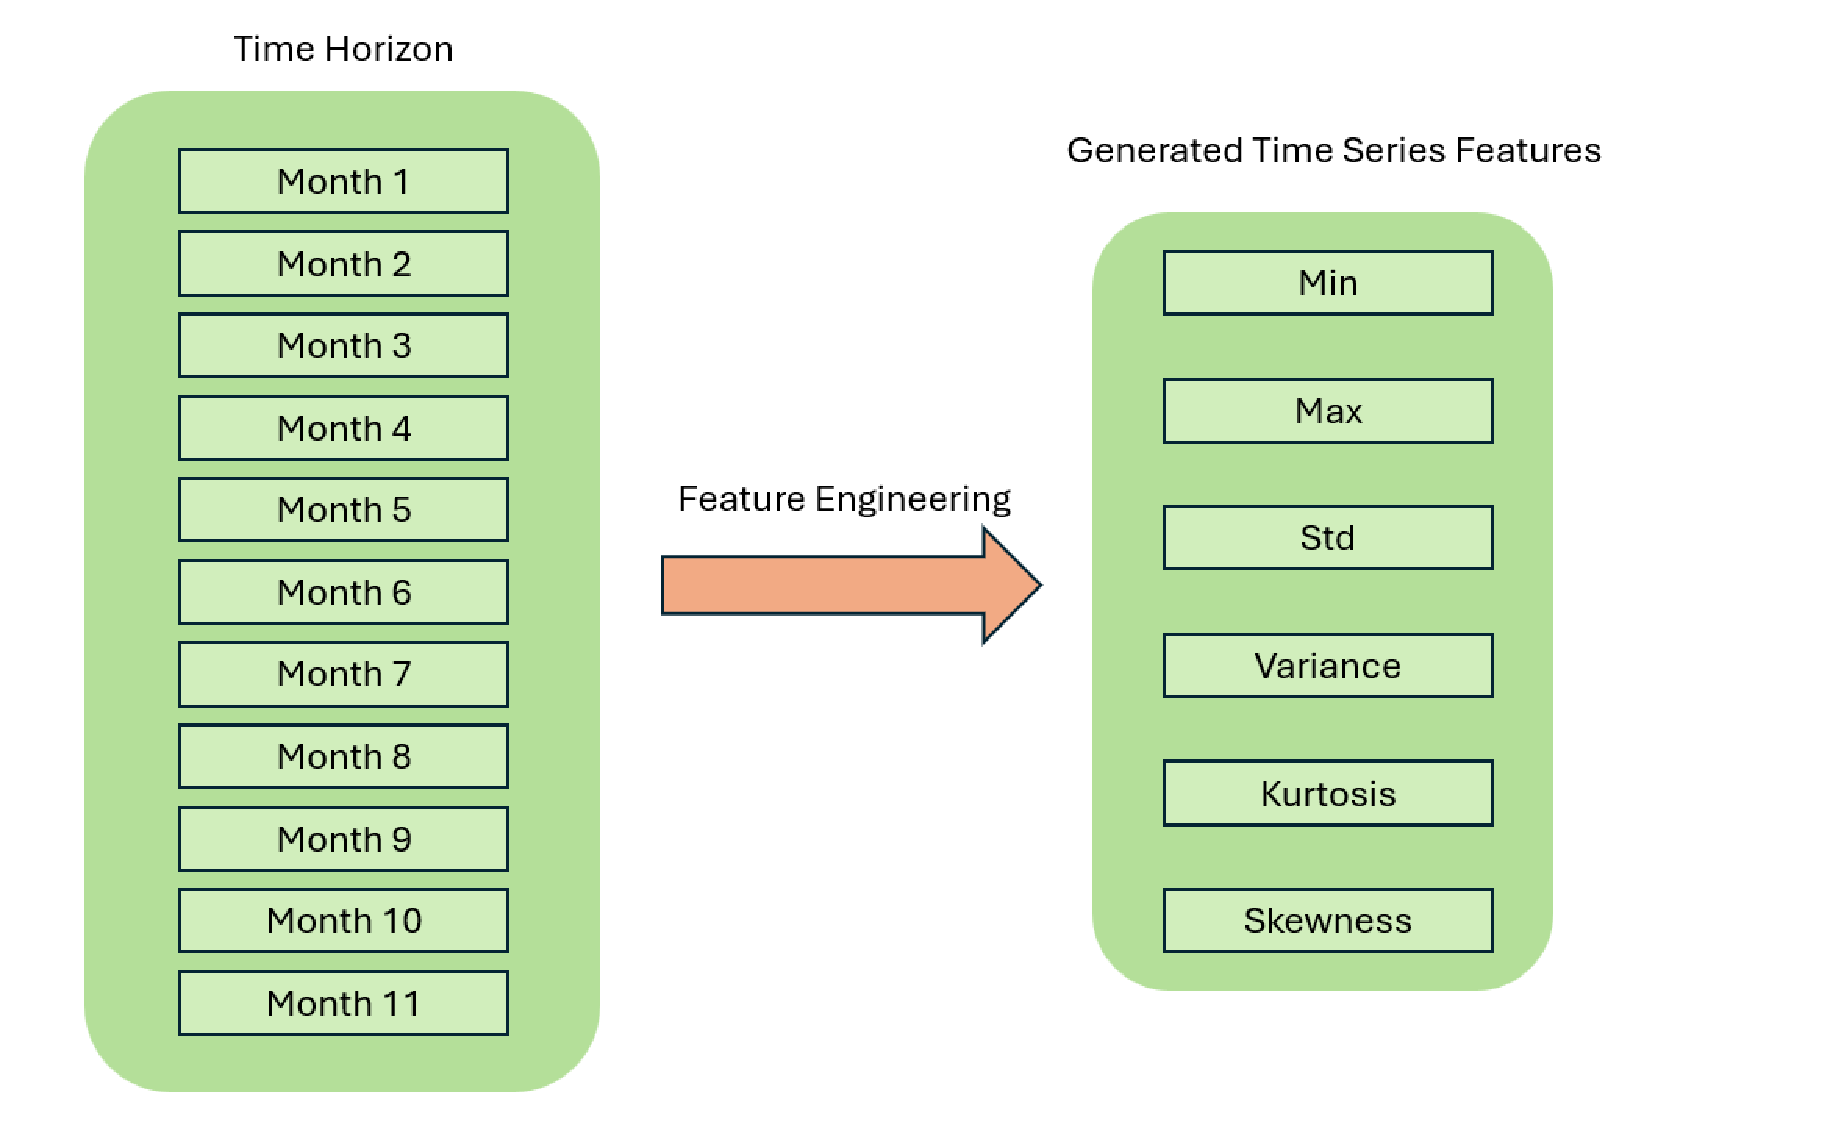
\includegraphics[width=0.9\linewidth]{Time_Series_Feature_Generation.pdf}
  \caption{Extraction of statistical and temporal features from the 10-month spectral time series.}
  \label{fig:ts_features}
\end{figure}

Table~\ref{tab:features} lists the time-series features extracted from each pixel's 10-month spectral profile \cite{mann2023}. This toolkit allowed us to extract all required time-series features efficiently, ensuring each pixel’s temporal signature was well-represented for robust classification \cite{mann2025}.


\begin{table}[htbp]
\centering
\small
\caption{Extracted time-series features.}
\label{tab:features}
\renewcommand{\arraystretch}{1.15}
\begin{tabular}{@{}>{\raggedright\arraybackslash}p{0.30\textwidth}p{0.62\textwidth}@{}}
\toprule
\textbf{Feature} & \textbf{Description} \\
\midrule
Absolute Energy & Sum of squared values, capturing overall signal magnitude. \\
Absolute Sum of Changes & Total absolute difference between consecutive measurements, reflecting temporal variability. \\
Autocorrelation (1, 2-month lag) & Correlation with its one- and two-month lagged versions, indicating series persistence. \\
Count Above Mean & Number of points above the series mean, quantifying high-value occurrences. \\
Day of Year of Max/Min & Julian day when the maximum and minimum occur, marking peak and low activity periods. \\
Kurtosis & Tail heaviness of the distribution, highlighting propensity for extremes. \\
Linear Trend & Slope of a least-squares fit, summarizing the overall upward or downward trend. \\
Longest Strike Above/Below Mean & Longest consecutive run above or below the mean, capturing sustained periods. \\
Max/Min & Absolute extreme values in the series. \\
Mean/Median & Measures of central tendency. \\
Mean Absolute Change/Mean Change & Average magnitude and signed change between consecutive points. \\
Mean Second Derivative & Mean of the series' second differences, detecting acceleration or deceleration. \\
Quantiles (0.05, 0.95) & Values at the 5th and 95th percentiles, summarizing distribution extremes. \\
Ratio Beyond \(r\sigma\) & Proportion of points more than \(r\) standard deviations ($r=1,2,3$) from the mean. \\
Skewness & Asymmetry of the distribution around the mean. \\
Standard Deviation/Variance & Spread measures around the mean. \\
Sum of Values & Total sum of observations (mean $\times$ length). \\
Symmetry Looking & Similarity when the series is reversed. \\
Time Series Complexity & Complexity-Invariant Distance metric of sequence irregularity. \\
\bottomrule
\end{tabular}

\par\vspace{4pt}
{\footnotesize Time-series features extracted from each pixel's spectral profile with \texttt{xr\_fresh}.\par}
\end{table}

\subsubsection{Pixel-Level Analysis}

For pixel-level analysis, each pixel was treated as an independent observation. Feature vectors from each pixel’s 10-month history were used to train classifiers. During inference, pixel predictions within a field polygon were aggregated via majority voting to determine the overall field label.

\paragraph{Baseline Classical Models.}

To benchmark crop classification, we used four classical models: Logistic Regression, Random Forest, LightGBM, and XGBoost, ranging from interpretable linear models to advanced tree-based learners. Each pixel was represented by a feature vector $\mathbf{x}_i \in \mathbb{R}^{174}$, formed from time-series features across ten months and six spectral bands and indices (B2, B6, B11, B12, EVI, Hue), capturing phenological signatures over time. These four models are standard and we summarize only their configurations here;
their formal definitions are collected in Appendix~\ref{app:models}.
Logistic Regression \cite{james2013} is a linear multinomial classifier
providing interpretable per-class weights. Random Forest \cite{breiman2001}
is a bagged ensemble of decision trees whose axis-aligned splits capture non-linear
interactions; we used 300 trees. LightGBM \cite{ke2017} and
XGBoost \cite{chen2016, friedman2001} are gradient-boosted tree ensembles
with leaf-wise growth and explicit $L_1$/$L_2$ regularization; both were trained with
GPU histogram methods. All four operate on the same per-pixel \texttt{xr\_fresh}
feature vector and, being tree- or margin-based with built-in feature selection or
shrinkage, serve as the parsimonious baselines against which the deep models are
compared.

\paragraph{Pixel-Level Ensemble with Hybrid Voting.}

We ensembled RF, XGBoost, and LightGBM using soft voting. Per-pixel class probabilities were averaged:
\[
\hat{\mathbf{P}}_i = \frac{1}{3} \left( \mathbf{P}_{\text{RF}}(\mathbf{x}_i) + \mathbf{P}_{\text{XGB}}(\mathbf{x}_i) + \mathbf{P}_{\text{LGBM}}(\mathbf{x}_i) \right)
\quad
\hat{y}_i = \arg\max_k \hat{P}_i(k)
\]

\paragraph{Field-Level Aggregation.}

Let field \( f \) consist of pixels \( i \in f \). Field-level soft voting is computed as:

\[
\bar{\mathbf{P}}_f = \frac{1}{|f|} \sum_{i \in f} \hat{\mathbf{P}}_i
\quad
\hat{y}_f^{\text{soft}} = \arg\max_k \bar{P}_f(k)
\]

We introduced a confidence margin:
\[
\Delta_f = \bar{P}_f^{(1)} - \bar{P}_f^{(2)}
\]

where \(\bar{P}_f^{(1)}\) and \(\bar{P}_f^{(2)}\) are the highest and second-highest class probabilities in \(\bar{P}_f\), respectively.\\

If \( \Delta_f < \theta \) (threshold = 0.10), we fall back to mode voting across pixel labels:

\[
\hat{y}_f^{\text{mode}} = \text{mode} \left\lbrace \hat{y}_i \mid i \in f \right\rbrace
\]

\paragraph{Final Hybrid Rule.}
\[
\hat{y}_f =
\begin{cases}
\hat{y}_f^{\text{soft}}, & \text{if } \Delta_f \geq \theta \\
\hat{y}_f^{\text{mode}}, & \text{otherwise}
\end{cases}
\]

This strategy balanced probabilistic confidence with categorical consistency, improving field-level classification stability.

\subsubsection{Field-Level Analysis}
In the field-level analysis, we aggregated all pixel features within each field polygon, as shown in Figure~\ref{fig:field_aggregation}, by computing the mean across pixels to form a single representative feature vector per field. This step reduced noise and the influence of outlier pixels while preserving meaningful spatial patterns. Classifiers were then trained using these aggregated field-level vectors to directly learn from spatially coherent crop representations. This approach aligns with previous findings that object-based aggregation helps in minimizing spectral confusion and enhances classification accuracy, especially in homogeneous agricultural regions \cite{penabarragan2011}.

\begin{figure}[htbp]
\centering
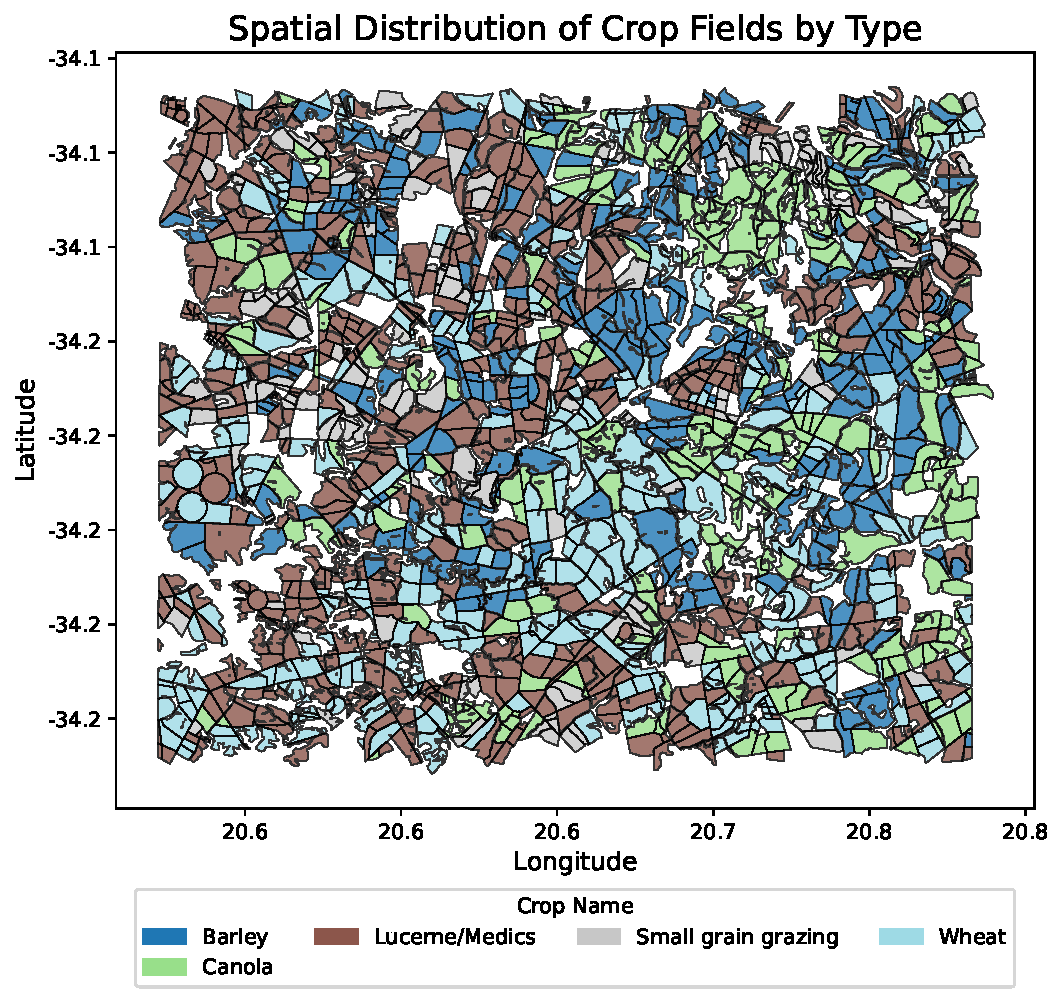
\includegraphics[width=0.9\linewidth]{field_boundaries_by_crop.pdf}
\caption{Field-level aggregation of pixel features.}
\label{fig:field_aggregation}
\par\vspace{4pt}
{\footnotesize Pixel values are grouped by field polygon and summarized into a single feature vector per field.\par}
\end{figure}

\vspace{0.5em}

To address class imbalance at the field level, we combined SMOTETomek resampling with a stacked ensemble classifier. This approach ensured both balanced data and strong generalization performance.
\paragraph{SMOTETomek Resampling.}
    SMOTETomek combines oversampling and undersampling techniques. SMOTE generates synthetic samples for underrepresented classes by interpolating between existing samples, while Tomek Links removes borderline examples to improve class separability. This helped mitigate the severe class imbalance visible in Figure~\ref{fig:EDA-1}, especially for crops like small-grain grazing and canola.\\

\paragraph{Stacked Ensemble Classifier.}
    We built a two-layer ensemble consisting of Random Forest and XGBoost as base learners, with Logistic Regression as the meta-learner, allowing it to use both base-model predictions and the original input features. The final prediction for pixel \(i\) is defined as:
    \[
    \hat{y}_i^{\text{stacked}} = f_{\text{meta}}\left(f_{\text{RF}}(\mathbf{x}_i),\; 
    f_{\text{XGB}}(\mathbf{x}_i),\; \mathbf{x}_i\right)
    \]
    This architecture combines the non-linear modeling capacity of tree-based learners with a linear meta-learner that integrates both base predictions and original input features.\\
We report this stacked ensemble in two forms that share the architecture above and differ only in resampling: \emph{SMOTE Stacked}, trained on SMOTETomek-resampled data as described, and \emph{Stacking}, the identical pipeline without resampling, so the pair isolates the effect of class rebalancing on spatial transfer.\\

\paragraph{Field-Based Aggregation and XGBoost Optimization.}
    We also implemented an optimized field-level pipeline using XGBoost. Field identifiers were used to ensure that no field contributed to more than one data split, with fields split into train/validation/test sets at the field level. Features were aggregated via the mean across pixels, and labels via the mode crop type per field.

Optuna was then used to tune XGBoost over 150 trials, searching over the number of trees, tree depth, learning rate, row and column subsampling fractions, minimum split loss, minimum child weight, and $L_1$ and $L_2$ regularization strengths, with the objective of maximizing the macro-averaged F1 score via 5-fold stratified cross-validation. The best configuration (Trial 32) is detailed in Table~\ref{tab:top5_trials}, which also achieved a validation accuracy of 76.61\%.

\begin{table}[htbp]
\centering
\scriptsize % Further reduce font size
\caption{XGBoost hyperparameter search results.}
\label{tab:top5_trials}
\renewcommand{\arraystretch}{1.1}
\setlength{\tabcolsep}{3pt} % Tight column spacing
\begin{tabular}{ccccccccccc}
\toprule
\textbf{Trial} & \textbf{Acc.} & \textbf{Est.} & \textbf{Depth} & \textbf{LR} & \textbf{SubS} & \textbf{ByTree} & \textbf{Gamma} & \textbf{Reg$\alpha$} & \textbf{Reg$\lambda$} & \textbf{MinCW} \\
\midrule
32 & \textbf{76.61\%} & 1141 & 13 & 0.0215 & 0.5749 & 0.6986 & 0.5589 & 0.00184 & 0.00259 & 5 \\
12 & 76.46\% & 984  & 12 & 0.0145 & 0.6675 & 0.6946 & 0.0799 & 0.00503 & 0.00455 & 7 \\
24 & 76.40\% & 1165 & 11 & 0.0162 & 0.7831 & 0.6403 & 0.00413 & 0.00481 & 0.00478 & 9 \\
13 & 76.29\% & 995  & 12 & 0.0277 & 0.6345 & 0.6829 & 0.3999 & 0.00011 & 0.00567 & 6 \\
18 & 76.29\% & 915  & 13 & 0.0121 & 0.6784 & 0.5958 & 0.1612 & 0.00491 & 0.1732 & 8 \\
\bottomrule
\end{tabular}

\par\vspace{4pt}
{\footnotesize Top 5 trials from the hyperparameter search with corresponding parameters and
validation accuracies. Bold marks the highest validation accuracy (trial 32).\par}
\end{table}

\subsection{Deep Learning Architectures}

Deep learning models ingest raw spectral values and learn hierarchical representations
that capture both spatial and temporal dependencies, offering an alternative to the
manual feature engineering required by classical approaches~\cite{zhu2017, tempcnn2019, russwurm2018, cnn_multitemp}.
We explore architectures across two spatial granularities: pixel-level models that
operate on per-pixel temporal sequences, and patch-level models that additionally
exploit local spatial structure. To ensure unbiased evaluation across all architectures,
all pixels belonging to a given field were assigned exclusively to either the training,
validation, or test set, preventing spatial information leakage between splits.

% ---------------------------------------------------------------
\subsubsection{Pixel-Level Architectures}
% ---------------------------------------------------------------

At the pixel level, each observation is an individual pixel characterized by 60 temporal
features spanning the 2017 growing season: six spectral bands and vegetation
indices (B2, B6, B11, B12, EVI, Hue) observed across 10 monthly composites.
Each pixel is linked to a unique field identifier and labeled according to the
field crop type across five classes: wheat, barley, canola, small-grain grazing,
and lucerne/medics. Two consequences of this design should be kept in mind. First,
pixels within a field are highly spatially autocorrelated and all inherit the same
field label (including mixed pixels along field boundaries), so although the
pixel-level models are trained on millions of observations, the number of statistically
independent units is closer to the number of fields than the number of pixels, and
the pixel models' apparent data volume overstates the effective training size.
Second, to prevent leakage we perform all train/validation/test splitting at the
field level, so no field's pixels straddle two partitions; this keeps
evaluation honest at the field scale even though training treats pixels as
independent. Pixel-level predictions are subsequently aggregated to the
field level via majority voting:
\[
    \hat{y}_{f} = \operatorname{mode}\!\left(\{\hat{y}_{i} \mid i \in f\}\right)
\]
For TabNet models we applied z-score standardization; CNN-based models were
trained on raw reflectance values, allowing convolutional layers to learn directly
from temporal magnitude patterns.

% --- 1. CNN + BiLSTM ---
\paragraph{CNN + BiLSTM Ensemble with Focal Loss.}

To capture the intricate temporal dynamics of crop growth, we developed a hybrid
architecture combining 1D Convolutional Neural Networks (CNNs) with Bidirectional
Long Short-Term Memory (BiLSTM) networks (Figure~\ref{fig:cnn_bilstm}).

\begin{figure}[htbp]
\centering
\includegraphics[width=0.9\textwidth]{cnn_bilstm.pdf}
\caption{Architecture of the CNN + BiLSTM model.}
\label{fig:cnn_bilstm}
\par\vspace{4pt}
{\footnotesize 1D convolutional temporal feature extraction is combined with sequential modeling through a BiLSTM layer.\par}
\end{figure}

The model processes an input tensor of shape $(B, 6, T)$. A 1D convolutional
layer with 64 filters and kernel size 5 is applied along the temporal axis,
followed by ReLU activation and tensor permutation to $(B, T, 64)$ for
compatibility with the recurrent layer. A bidirectional LSTM with hidden size
64 then captures temporal dependencies in both forward and backward directions,
yielding an output of shape $(B, T, 128)$. The representation at the final
timestep passes through dropout and a fully connected layer, with class
probabilities computed via softmax:
\[
    P(y_i = c \mid \mathbf{x}_i)
    = \frac{e^{z_{i,c}}}{\sum_{c'=1}^{C} e^{z_{i,c'}}}
\]

To address class imbalance we used Focal Loss:
\[
    \mathcal{L}_{\text{focal}} = -\alpha_t (1 - p_t)^{\gamma} \log(p_t)
\]
where $\alpha_t$ is a per-class weight set to the inverse class frequency and
$\gamma = 2.0$ is the focusing parameter, so class imbalance is handled directly in
the loss rather than by resampling. To reduce variance, five
identical models were trained with different random seeds and their logits averaged:
\[
    \text{Logits}_{\text{ensemble}}
    = \frac{1}{N} \sum_{k=1}^{N} \text{Logits}^{(k)}
\]

% --- 2. TabNet ---
\paragraph{TabNet with Sparsemax Feature Masks.}

TabNet treats satellite observations as structured tabular inputs (each pixel's
repeated measurements organized as a flat feature vector) and learns through
iterative attention-based feature selection rather than temporal ordering. At each
of $n_{\text{steps}}$ decision steps, an Attentive Transformer produces a sparse feature
mask via \emph{sparsemax},
\[
  \mathbf{M}[i]=\operatorname{sparsemax}\!\big(\mathbf{P}[i-1]\odot h_i(\mathbf{a}[i-1])\big),
  \qquad
  \mathbf{P}[i]=\prod_{j=1}^{i}\big(\gamma-\mathbf{M}[j]\big),
\]
where $h_i$ is a trainable transform of the previous step's processed features
$\mathbf{a}[i-1]$ and the prior scale $\mathbf{P}$ enforces the relaxation $\gamma$ that
discourages re-selecting the same features across steps; the masked features
$\mathbf{M}[i]\odot\mathbf{f}$ are then handled by a Feature Transformer. This lets the
model focus on different feature subsets at different depths without relying on explicit
temporal structure~\cite{tabnet_orig, tabnet2024}, and this sparsemax feature-mask
mechanism is precisely what the L-TAE-S (below) grafts onto a temporal-attention backbone.

The network used $n_d = n_a = 64$, 2 independent and 2 shared feature-transformer blocks,
relaxation parameter $\gamma = 1.5$, and 5 decision steps. Training used the
Adam optimizer with a step-decay learning-rate schedule, batch size 1024, virtual batch size
128, and early stopping monitored on a field ID-stratified validation set.

An ensemble of five TabNet models, each initialized with a distinct random seed
(42, 101, 202, 303, 404), averaged softmax outputs to yield final class
probabilities:
\[
    \hat{\mathbf{p}}_{\text{ensemble}}
    = \frac{1}{5}\sum_{i=1}^{5}\operatorname{Softmax}\!\left(\mathbf{z}^{(i)}\right),
    \qquad
    \hat{y} = \arg\max_c\,\hat{p}_{\text{ensemble},c}
\]
A practical advantage of TabNet is interpretability: the sparse decision masks
can be inspected post hoc to identify which spectral bands or vegetation indices
most influenced each prediction~\cite{tabnet2024}, an instance of the post-hoc explainability increasingly emphasized in remote sensing~\cite{hohl2024}.

% --- 4. L-TAE ---
\paragraph{Lightweight Temporal Attention Encoder (L-TAE).}

The L-TAE applies self-attention directly to the temporal sequence of per-pixel
reflectance vectors, learning which observations in the season are most informative
\cite{ltae2020}. Given the embedded sequence $\{\mathbf{z}_t\}_{t=1}^{T}$, a set of
learned master query vectors attend over time; for a single head the output is a
temporally weighted sum
\[
    \mathbf{o} = \sum_{t=1}^{T}\alpha_t\,\mathbf{v}_t,
    \qquad
    \alpha_t = \frac{\exp\!\big(\mathbf{q}^\top\mathbf{k}_t/\sqrt{d}\big)}
                    {\sum_{t'=1}^{T}\exp\!\big(\mathbf{q}^\top\mathbf{k}_{t'}/\sqrt{d}\big)},
\]
where $\mathbf{k}_t,\mathbf{v}_t$ are key/value projections of $\mathbf{z}_t$,
$\mathbf{q}$ is the learned query, and $d$ is the head dimension. Channel grouping
keeps the encoder lightweight. We evaluated L-TAE both at the pixel level and at the
field level (averaging pixel sequences within a field before encoding), and trained a
five-seed ensemble.

% --- 4a. Transformer encoder ---
\paragraph{Pixel-Level Transformer Encoder.}

As a dense-attention reference point we evaluated a standard Transformer encoder applied
to the per-pixel reflectance sequence \cite{vaswani2017, russwurm2020}. After the same
linear band embedding and sinusoidal positional encoding used for the L-TAE (with the
true month indices, so the May--June gap is preserved), the embedded sequence
$\mathbf{Z}=[\mathbf{z}_1,\dots,\mathbf{z}_T]$ passes through three pre-norm multi-head
self-attention layers, each computing
\[
  \operatorname{head}_i=\operatorname{softmax}\!\Big(
    \tfrac{(\mathbf{Z}W_i^{Q})(\mathbf{Z}W_i^{K})^{\top}}{\sqrt{d_k}}\Big)\mathbf{Z}W_i^{V},
  \qquad
  \operatorname{MHSA}(\mathbf{Z})=\big[\operatorname{head}_1\,\Vert\cdots\Vert\,
    \operatorname{head}_{8}\big]\,W^{O},
\]
with $d_{\text{model}}=128$, $8$ heads, and feed-forward width $256$; unlike the L-TAE's
single learned query, every time step here attends to every other. The encoded time steps
are mean-pooled and passed to a two-layer classification head. This makes it the most expressive attention
model we evaluate; yet, unlike the L-TAE-S below, it contains no feature-sparsity
mechanism. It therefore serves as a control that
separates attention \emph{capacity} from feature \emph{sparsity}. We trained it at the
pixel level as a five-seed ensemble under the same weighted-focal-loss objective and
field-aggregation protocol as the other temporal models.

% --- 4b. Sparse-attention L-TAE ---
\paragraph{Sparse-Attention L-TAE (L-TAE-S).}

To test whether a tree-like, sparse inductive bias can be grafted onto the temporal
attention encoder, we implemented a sparse-attention variant (L-TAE-S) that inserts a
TabNet-inspired channel-selection gate before the attention heads (Figure~\ref{fig:ltae_s}). For each of the
$n_{\text{head}}=16$ heads, a per-head linear projection of the embedded sequence
($d_{\text{model}}=128$) is passed through \emph{sparsemax}~\cite{sparsemax2016} to
produce a sparse, instance-dependent mask over the embedding channels, so each head
attends to a small learned subset of features (with key dimension $d_k=8$). The
TabNet-style relaxation prior uses $\gamma=1.5$ and the sparsity weight is
$\lambda=10^{-3}$; the resulting masks (which can be time-varying) are differentiable and
interpretable, mirroring TabNet's sparsemax feature masks~\cite{tabnet_orig} while
retaining the temporal-attention backbone of the L-TAE~\cite{ltae2020}.
Formally, for head $h$ and embedded, positionally-encoded time step
$\mathbf{z}_t\in\mathbb{R}^{E}$ (with $E=d_{\text{model}}$), the gate produces a sparse
channel mask $\mathbf{m}_{h,t}$ and a masked embedding $\tilde{\mathbf{z}}_{h,t}$,
\[
  \mathbf{m}_{h,t}=\operatorname{sparsemax}\!\big(\mathbf{P}_{h,t}\odot
    \operatorname{BN}(W_h\mathbf{z}_t)\big),\qquad
  \tilde{\mathbf{z}}_{h,t}=\mathbf{m}_{h,t}\odot\mathbf{z}_t,\qquad
  \mathbf{P}_{h+1,t}=\mathbf{P}_{h,t}\odot\max(\gamma-\mathbf{m}_{h,t},\,0),
\]
initialized at $\mathbf{P}_{1,t}=\mathbf{1}$; head $h$ then forms its keys and values from
$\tilde{\mathbf{z}}_{h,t}$ before applying the L-TAE attention above. Because
\emph{sparsemax} projects onto the probability simplex, most channels of
$\mathbf{m}_{h,t}$ are exactly zero, and the relaxation prior $\mathbf{P}_{h,t}$
(coefficient $\gamma$) discourages successive heads from re-selecting the same channels;
a penalty $\lambda\sum_{h,t}\lVert\mathbf{m}_{h,t}\rVert_{1}$ adds mild additional
pressure. (We use
\emph{sparsemax}; the $\alpha$-entmax family~\cite{entmax2019} generalizes it with a
tunable sparsity level and is a natural alternative we leave to future work.) We evaluate
L-TAE-S as a first-class model at both the pixel and field level (a five-seed ensemble
trained under the same weighted-focal-loss objective and field-aggregation protocol as the
other temporal networks) and find that this single architectural change makes it one of
the most transferable models in the study (Tables~\ref{tab:gap}--\ref{tab:pixfield};
Section~\ref{subsec:featdim}).

\begin{figure}[htbp]
\centering

\includegraphics[width=\linewidth]{ltae_s.pdf}
\caption{Architecture of the sparse-attention L-TAE-S.}
\label{fig:ltae_s}
\par\vspace{4pt}
{\footnotesize Each ensemble member embeds the per-pixel Sentinel-2 time series, adds
month-aware positional encoding, and, before the multi-head temporal attention,
applies a TabNet-style \emph{sparse feature gate} (highlighted): a per-head
\texttt{sparsemax} mask selects a small subset of embedding channels, with a relaxation
prior ($\gamma=1.5$) discouraging heads from re-selecting the same channels. This single
block, which grafts a tree-like sparse feature-selection inductive bias onto the attention
backbone, is the only architectural difference from the L-TAE. Five seeds are ensembled
and aggregated to field level.\par}
\end{figure}

% --- 5. TempCNN ---
\paragraph{Temporal Convolutional Network (TempCNN).}

TempCNN classifies a pixel from stacked one-dimensional convolutions applied along the
temporal axis, each capturing local phenological motifs of increasing receptive field
\cite{tempcnn2019}. A convolutional layer computes
\[
    h^{(l)}_{t} = \operatorname{ReLU}\!\Big(\operatorname{BN}\big(
        \textstyle\sum_{\tau=-k}^{k} W^{(l)}_{\tau}\,h^{(l-1)}_{t+\tau} + b^{(l)}\big)\Big),
\]
with batch normalization (BN) and dropout for regularization, followed by a fully
connected softmax head. As with L-TAE, we evaluated pixel- and field-level variants
and ensembled across five seeds.

% ---------------------------------------------------------------
\subsubsection{Patch-Level Architectures}
% ---------------------------------------------------------------

To exploit local spatial structure, we transitioned to a patch-level analysis in
which each field is tiled into 100\,m square patches ($\approx$10$\times$10 pixels at
the 10\,m resolution), each retaining the full 10-month spectral history for every
pixel (Figure~\ref{fig:example_patches}). Fields smaller than one hectare are kept
whole as a single patch, and grid patches not fully contained within a field are
discarded to avoid mixed-boundary pixels. Because the median field (7--11\,ha) is
several times larger than a patch, most fields yield several patches, providing
implicit data augmentation. Before entering the convolutional models, each patch is
resampled to a fixed $128\times128$ grid; we note that this upsamples the native
$\sim$10$\times$10-pixel patches by roughly an order of magnitude, so the enlarged
input reflects interpolation rather than additional spatial detail.

\begin{figure}[H]
\centering
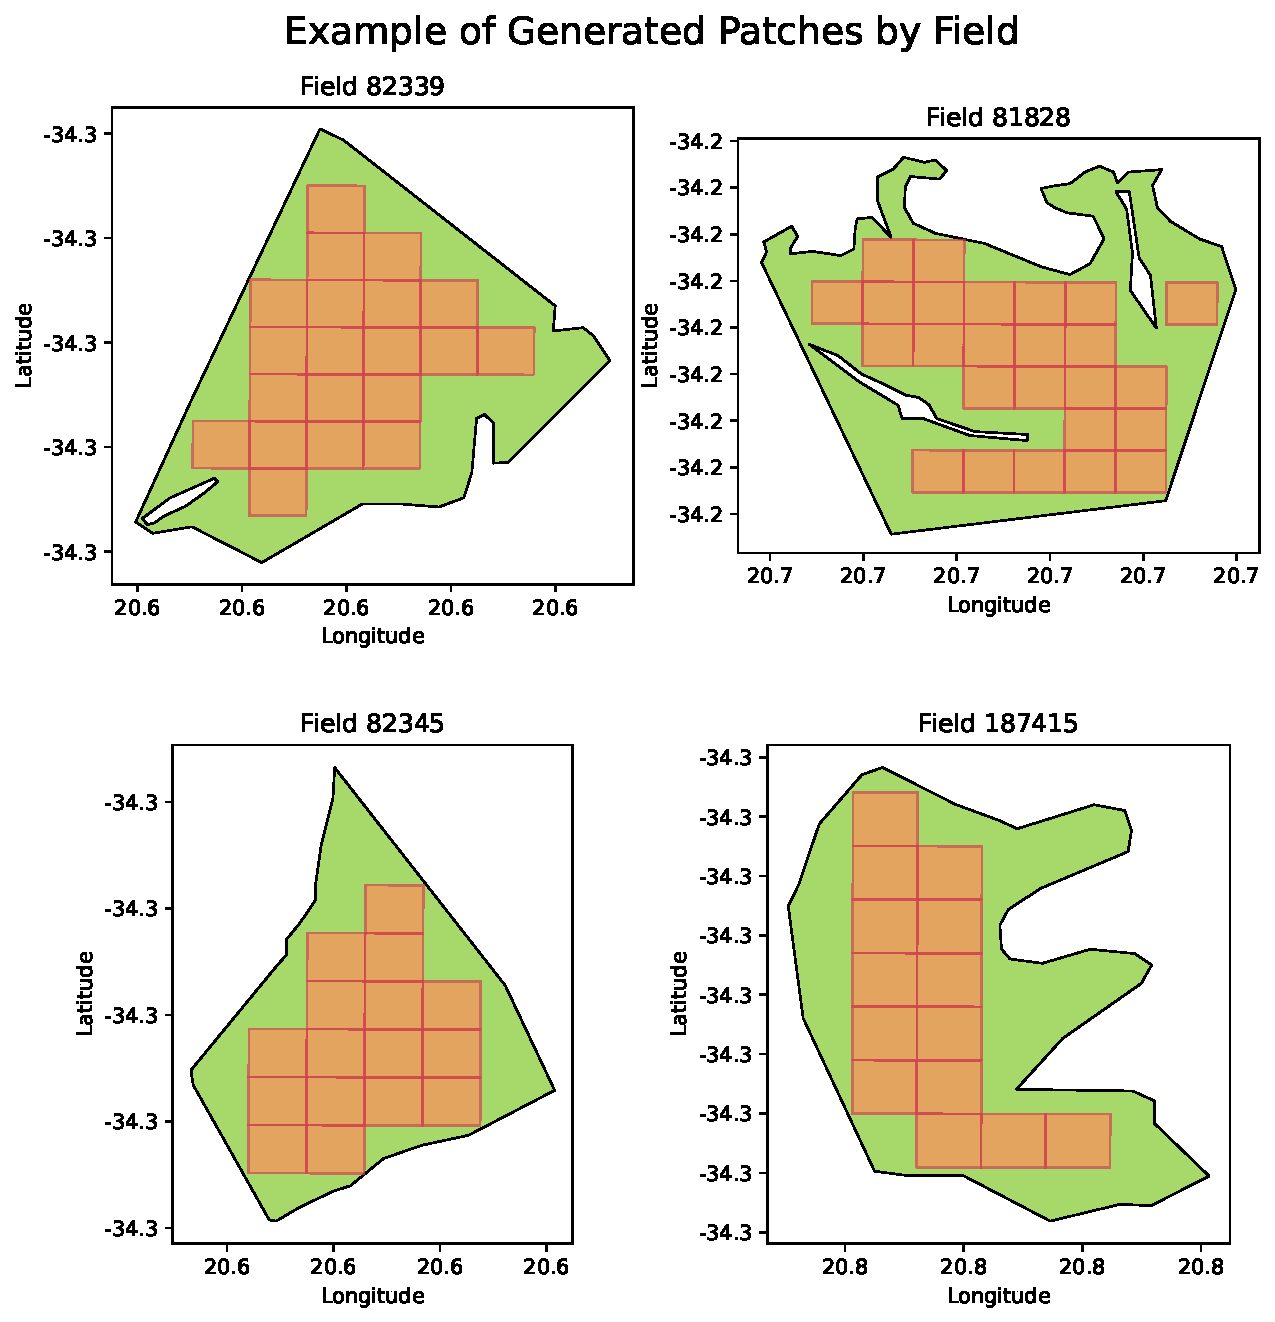
\includegraphics[width=0.9\linewidth]{Example_patches.pdf}
\caption{Illustration of patch generation per field.}
\label{fig:example_patches}
\end{figure}

We investigated two distinct patch-based architectures.

% --- 3a. Multi-Channel 2D CNN ---
\paragraph{Multi-Channel 2D CNN.}

Each spectral band and monthly observation is treated as a separate input channel,
giving a patch tensor $\mathbf{X} \in \mathbb{R}^{H \times W \times C}$
($H = W = 128$ after resampling, $C = 60 = 6\text{ features} \times 10\text{ months}$).
Two 2D-convolutional blocks ($32$ and $64$ filters, $3\times3$ kernels), each followed by
max-pooling, compute (for filter $k$):
\[
    Y_k[i,j] = \operatorname{ReLU}\!\left(
        \sum_{c=1}^{C}\sum_{m=-1}^{1}\sum_{n=-1}^{1}
        W_{k,c,m,n}\cdot X[i+m,\,j+n,\,c] + b_k
    \right)
\]
The pooled feature map is flattened and projected by a dense hidden layer to
$\mathbf{z} \in \mathbb{R}^{64}$ (ReLU), then passed to a fully connected
classification head:
\[
    \hat{\mathbf{p}} = \operatorname{softmax}\!\left(W_{\mathrm{fc}}\,\mathbf{z} + b_{\mathrm{fc}}\right)
\]

% --- 3b. Ensemble of Class-Specific 3D CNNs ---
\paragraph{Ensemble of Class-Specific 3D CNNs.}

Five class-specific 3D CNNs are trained, each producing a scalar score
$p_i = f_i(\mathbf{X})$ for its target class. A logistic regression meta-learner
combines these scores into a final prediction (Figure~\ref{fig:patch_model}):
\[
    \hat{\mathbf{p}} = \operatorname{softmax}\!\left(
        W_{\mathrm{meta}}[p_1,\dots,p_5]^\top + b_{\mathrm{meta}}
    \right)
\]
By modelling volumetric relationships jointly across spectral bands, spatial
dimensions, and time, 3D convolutions capture crop-specific texture and
phenological trajectories that 2D methods treat independently.

\begin{figure}[htbp]
\centering
\includegraphics[width=0.9\linewidth]{patch_model.pdf}
\caption{3D CNN ensemble architecture for patch-level crop classification.}
\label{fig:patch_model}
\end{figure}

\subsection{Performance Metrics}
\label{subsec:performance_metrics}

Because the class distribution is severely imbalanced (Figure~\ref{fig:EDA-1}),
plain accuracy is misleading: a classifier can score highly simply by predicting
the majority class. We therefore adopt macro-averaged F1 (F1$_m$), the
unweighted mean of the per-class F1 scores, as our primary metric: it weights
every crop equally and so directly penalizes failure on the minority cereals, which
is exactly where models differ. We report three further metrics alongside it:
Cohen's Kappa, chance-corrected agreement between predicted and true labels;
weighted F1, the support-weighted mean of per-class F1; and cross-entropy
(Xent), the field-level cross-entropy that served as the official scoring metric of the
AI4FoodSecurity (South Africa) challenge~\cite{ai4foodsecurity} from which our dataset is
drawn (lower is better; computed on hard crop-label predictions, Appendix~\ref{app:metrics}).
Higher Kappa and F1 indicate
better, more balanced classification. Formal definitions of all four metrics are
given in Appendix~\ref{app:metrics}.

\section{Results}
\label{sec:results}

We evaluated every model under two protocols. \emph{In-region field-wise validation} uses a
field-wise train/validation/test split drawn entirely
from the training tiles, this is the conventional way crop classifiers are benchmarked;
we shorten this to ``in-region''. \emph{Spatial transfer} (ST) applies the trained model to the spatially
disjoint holdout tile (\texttt{34S\_20E\_259N}; 2{,}417 fields). All predictions
are aggregated to the field level. Because the classes are heavily imbalanced
(Section~\ref{subsec:performance_metrics}), we report macro-averaged F1
(F1$_m$) as the primary metric, with Cohen's Kappa, weighted F1, and log-loss
(cross-entropy) alongside.

\subsection{In-region validation overstates performance and misranks models}

Table~\ref{tab:gap} reports both protocols for all individual models, ranked by
spatial-transfer macro-F1, with the spatial-transfer gap
$\Delta = \text{F1}_m^{\text{ST}} - \text{F1}_m^{\text{in-region}}$ shown alongside;
Figure~\ref{fig:gap} visualizes the same data ordered by $\Delta$. Two facts stand out. First, \emph{every}
model loses accuracy under spatial transfer, but the loss is highly uneven: it ranges from
$-0.04$ (the field-level sparse-attention L-TAE-S) to $-0.26$ (CNN-BiLSTM at the pixel level).
Second, this unevenness reorders the models. Under in-region validation the dense temporal
pixel-level deep nets cluster at the top, with F1$_m$ scores for L-TAE at 0.78, Transformer 0.78, L-TAE-S 0.77,
TempCNN 0.77, CNN-BiLSTM 0.72. A reasonable practitioner choosing by in-region F1 would pick
from this cluster. On the holdout tile the cluster fractures sharply: the two in-region
leaders (L-TAE pixel and the Transformer encoder, $\Delta=-0.20$) drop to F1$_m=0.58$,
TempCNN ($-0.21$) to 0.56, and CNN-BiLSTM ($-0.26$) to 0.46, this is among the lowest absolute
scores of any model. Only L-TAE-S, the sparse-attention variant, holds its ground. The
same in-region-to-holdout collapse befalls the 3D CNN patch ensemble ($-0.22$), the
Multi-Channel 2D CNN ($-0.22$), and SMOTE-resampled stacking ($-0.21$).

\begin{table}[htbp]
\centering
\scriptsize
\caption{In-region versus spatial-transfer performance of all models.}
\label{tab:gap}
\renewcommand{\arraystretch}{1.12}
\setlength{\tabcolsep}{4pt}
\begin{tabular}{lllcccccc}
\toprule
 & & & \textbf{In-reg} & & \multicolumn{4}{c}{\textbf{Spatial transfer (ST)}} \\
\cmidrule(lr){4-4}\cmidrule(lr){6-9}
\textbf{Model} & \textbf{Level} & \textbf{Features} & \textbf{F1$_m$} & \textbf{$\Delta$} & \textbf{F1$_m$} & \textbf{$\kappa$} & \textbf{wF1} & \textbf{Xent} \\
\midrule
TabNet                & pixel & raw & 0.73 & $-0.13$ & \textbf{0.60} & \textbf{0.54} & 0.70 & \textbf{4.42} \\
L-TAE-S               & field & raw & 0.64 & $\mathbf{-0.04}$ & 0.60 & 0.52 & 0.69 & 4.77 \\
L-TAE-S               & pixel & raw & 0.77 & $-0.17$ & 0.60 & 0.53 & \textbf{0.70} & 4.63 \\
L-TAE                 & field & raw & 0.67 & $-0.07$ & 0.59 & 0.47 & 0.67 & 5.51 \\
L-TAE                 & pixel & raw & \textbf{0.78} & $-0.20$ & 0.58 & 0.49 & 0.68 & 5.20 \\
Transformer           & pixel & raw & \textbf{0.78} & $-0.20$ & 0.58 & 0.50 & 0.69 & 4.94 \\
XGBoost               & field & \texttt{xr\_fresh} & 0.70 & $-0.13$ & 0.56 & 0.47 & 0.68 & 4.89 \\
TempCNN               & pixel & raw & 0.77 & $-0.21$ & 0.56 & 0.49 & 0.68 & 5.09 \\
Base LightGBM         & pixel & \texttt{xr\_fresh} & 0.62 & $-0.06$ & 0.56 & 0.47 & 0.66 & 4.85 \\
Logistic Regression   & pixel & \texttt{xr\_fresh} & 0.61 & $-0.05$ & 0.56 & 0.47 & 0.67 & 4.93 \\
LightGBM              & field & \texttt{xr\_fresh} & 0.68 & $-0.12$ & 0.56 & 0.45 & 0.66 & 4.99 \\
Voting                & pixel & \texttt{xr\_fresh} & 0.65 & $-0.09$ & 0.56 & 0.48 & 0.66 & 4.85 \\
Random Forest         & pixel & \texttt{xr\_fresh} & 0.65 & $-0.10$ & 0.55 & 0.45 & 0.65 & 5.07 \\
Base XGBoost          & pixel & \texttt{xr\_fresh} & 0.64 & $-0.09$ & 0.54 & 0.47 & 0.66 & 5.01 \\
TempCNN               & field & raw & 0.67 & $-0.14$ & 0.54 & 0.43 & 0.64 & 6.07 \\
Stacking              & field & \texttt{xr\_fresh} & 0.64 & $-0.11$ & 0.53 & 0.48 & 0.67 & 5.32 \\
CNN-BiLSTM            & field & raw & 0.64 & $-0.14$ & 0.51 & 0.33 & 0.54 & 7.86 \\
SMOTE Stacked         & field & \texttt{xr\_fresh} & 0.69 & $-0.21$ & 0.49 & 0.43 & 0.63 & 5.37 \\
3D CNN                & patch & raw & 0.70 & $-0.22$ & 0.48 & 0.30 & 0.55 & 7.79 \\
CNN-BiLSTM            & pixel & raw & 0.72 & $-0.26$ & 0.46 & 0.32 & 0.56 & 7.73 \\
TabNet Temporal       & field & raw & 0.62 & $-0.19$ & 0.43 & 0.31 & 0.56 & 7.35 \\
Multi-Channel CNN     & patch & raw & 0.63 & $-0.22$ & 0.40 & 0.25 & 0.50 & 8.62 \\
TabNet                & field & \texttt{xr\_fresh} & 0.51 & $-0.15$ & 0.37 & 0.25 & 0.53 & 6.13 \\
\bottomrule
\end{tabular}

\par\vspace{4pt}
{\footnotesize In-region (field-wise validation) versus spatial-transfer (ST) macro-F1
for every individual model, ranked by spatial-transfer macro-F1, the metric we argue
model selection should use. In-region macro-F1 and the gap $\Delta$ are shown
alongside (Figure~\ref{fig:gap} orders the same data by $\Delta$); ST Kappa, weighted
F1 (wF1), and cross-entropy (Xent, the AI4FoodSecurity challenge's official field-level scoring metric~\cite{ai4foodsecurity}, lower is better) complete the picture. Bold marks the best value in
each metric column. The best transferer is a TabNet pixel ensemble; the highest in-region
scores (L-TAE and Transformer pixel, both $0.78$; L-TAE-S and TempCNN pixel, both $0.77$)
do not yield the highest spatial-transfer scores, and CNN-BiLSTM, singled out by prior
analysis of this dataset~\cite{capstone_repo}, suffers the largest drop of any model
($\Delta = -0.26$ at the pixel level). The \emph{Features} column
marks whether a model is fed the automated \texttt{xr\_fresh} time-series statistics
(174 features) or raw reflectance; the \texttt{xr\_fresh} models are the classical
learners: the four \emph{Base} models on per-pixel statistics, the field ensembles on
field-averaged statistics.\par}
\end{table}

\begin{figure}[htbp]
\centering

\includegraphics[width=\linewidth]{train_vs_oos_gap.pdf}
\caption{In-region versus spatial-transfer macro-F1 by model, sorted by gap.}
\label{fig:gap}
\par\vspace{4pt}
{\footnotesize In-region performance is from field-wise validation. Dense temporal/patch
deep nets (top) suffer the largest degradation; tree-based, linear, and field-aggregated
models (bottom) transfer with the smallest gaps.\par}
\end{figure}

The winners under spatial transfer are a different group entirely. The best single
model is the TabNet pixel ensemble (F1$_m=0.60$, Kappa 0.54), which also posts the lowest holdout cross-entropy on the challenge's official metric ($4.42$) of any model, tied on macro-F1 by both
sparse-attention L-TAE-S variants (F1$_m=0.60$; Section~\ref{subsec:featdim}). The most
\emph{robust} models, those with the smallest gaps, are the sparse learners: the
field-level L-TAE-S posts the single smallest gap of any model ($\Delta=-0.04$), just
ahead of logistic regression ($-0.05$), pixel-level LightGBM ($-0.06$), and the
pixel-level tree learners. That L-TAE-S sits at the top of the robustness ranking is itself evidence for our
thesis. It is a deep temporal attention network, but with one twist: a learned gate
restricts each attention head to a small subset of input channels rather than mixing
all of them. That built-in selectivity, copied directly from TabNet, is precisely
what gives it the cross-region stability the other deep nets lack. Notably, the robust \texttt{xr\_fresh} classical ensembles in the upper-middle of the
table (XGBoost, Voting, LightGBM, Stacking) are the models fed the
automated \texttt{xr\_fresh} features (Table~\ref{tab:gap}, Features column): the
combination of a rich automated feature representation with a tree learner transfers
well, whereas the deep nets that learn from raw sequences do not. The practical
implication is immediate: a user who picked by in-region F1$_m$ would have landed on
L-TAE, the Transformer encoder, or TempCNN (all 0.77--0.78 in-region), each of which
drops to 0.56--0.58 on the holdout and falls below TabNet (0.60). CNN-BiLSTM, the
model prior analysis of this dataset singled out~\cite{capstone_repo}, fares worse
still under transfer (F1$_m=0.46$, among the lowest absolute scores in the
benchmark).

\subsection{Pixel versus field level: aggregation as variance reduction}
\label{subsec:pixel_field}

Several architectures were run at both the pixel level and the field level (averaging
the per-pixel time series within each field before classification). Table~\ref{tab:pixfield}
and Figure~\ref{fig:pixfield} show that field-level aggregation acts as a
variance-reduction regularizer for the \emph{dense} temporal networks: L-TAE improves
from F1$_m=0.58$ (pixel) to $0.59$ (field) while its gap shrinks from $-0.20$ to
$-0.07$, and CNN-BiLSTM, the worst pixel-level transferer, recovers most of all when
field-trained, its gap halving from $-0.26$ to $-0.14$ (F1$_m$ $0.46\rightarrow0.51$).
TempCNN is a partial exception: its gap narrows from $-0.21$ to $-0.14$, but its
ST F1$_m$ slips slightly ($0.56\rightarrow0.54$), so the gap narrowing reflects a
drop in the in-region ceiling more than a holdout gain. The sparse-attention L-TAE-S follows
the same dense-backbone pattern despite its TabNet-style channel gating: its gap shrinks
from $-0.17$ (pixel) to $-0.04$ (field, the smallest of any model) while ST F1$_m$ holds
at $0.60$; so the temporal backbone, not the sparse gate, governs the response to
aggregation. Averaging pixels within a
field cancels region-specific pixel noise before the model sees it, lowering the
in-region ceiling and, for most dense models, improving transfer. TabNet is the informative exception:
aggregating its raw inputs to the field level \emph{hurts} (F1$_m$ falls from 0.60 to
0.43), because its robustness already derives from sparse feature selection and
field-level training starves it of the per-pixel observation volume it exploits (millions of
pixels versus a few thousand fields). The tree ensembles transfer well at either level.
In short, dense models need aggregation to generalize; sparse, tree-like models do not.

A second comparison is embedded in the same table. The tree learners are run at both
granularities on the \emph{same} \texttt{xr\_fresh} representation: the \emph{Base}
models (Logistic Regression, Random Forest, LightGBM, XGBoost) on per-pixel statistics,
and the field ensembles (XGBoost, LightGBM) on field-averaged statistics, so their
pixel$\rightarrow$field change isolates the effect of aggregation alone, with the
feature representation held fixed. That change is essentially neutral under spatial
transfer: XGBoost moves from F1$_m=0.54$ (pixel) to $0.56$ (field) and LightGBM stays at
$0.56$, even though aggregation raises the in-region score (e.g.\ XGBoost
$0.64\rightarrow0.70$) and therefore widens the gap. Aggregation thus adds little for
the already-sparse tree learners. Because every classical model here is built on
\texttt{xr\_fresh}, our experiments do not isolate the marginal value of the
\texttt{xr\_fresh} representation against raw reflectance for the trees; \texttt{xr\_fresh}'s
contribution is operational (it compresses each pixel's ten-month, six-band series into a
single compact vector that a tree fits in minutes) rather than a demonstrated gain in
spatial-transfer accuracy. TabNet, run at the field level with both raw field-averaged and
\texttt{xr\_fresh} inputs, behaves consistently: moving its raw inputs from pixel to field
level costs F1$_m$ $0.60\rightarrow0.43$ (the aggregation/observation-volume penalty), and the
field \texttt{xr\_fresh} variant is lower still at $0.37$. So for TabNet aggregation does
not help, consistent with the broader finding that already-sparse models gain nothing
from field-level averaging.

\begin{table}[htbp]
\centering
\caption{Pixel- versus field-level spatial transfer.}
\label{tab:pixfield}
\renewcommand{\arraystretch}{1.1}
\setlength{\tabcolsep}{5.5pt}
\begin{tabular}{lccccl}
\toprule
 & \multicolumn{2}{c}{\textbf{Pixel}} & \multicolumn{2}{c}{\textbf{Field}} & \\
\cmidrule(lr){2-3}\cmidrule(lr){4-5}
\textbf{Architecture} & \textbf{ST F1$_m$} & \textbf{$\Delta$} & \textbf{ST F1$_m$} & \textbf{$\Delta$} & \textbf{Field input} \\
\midrule
L-TAE-S    & \textbf{0.60} & $-0.17$         & \textbf{0.60} & $\mathbf{-0.04}$ & raw-avg \\
L-TAE      & 0.58          & $-0.20$         & 0.59          & $-0.07$         & raw-avg \\
XGBoost    & 0.54          & $-0.09$         & 0.56          & $-0.13$         & \texttt{xr\_fresh} \\
LightGBM   & 0.56          & $\mathbf{-0.06}$ & 0.56          & $-0.12$         & \texttt{xr\_fresh} \\
TempCNN    & 0.56          & $-0.21$         & 0.54          & $-0.14$         & raw-avg \\
CNN-BiLSTM & 0.46          & $-0.26$         & 0.51          & $-0.14$         & raw-avg \\
TabNet     & \textbf{0.60} & $-0.13$         & 0.43          & $-0.19$         & raw-avg \\
\bottomrule
\end{tabular}

\par\vspace{4pt}
{\footnotesize Spatial-transfer (ST) macro-F1 (and gap $\Delta$) at pixel versus field level for
architectures evaluated at both granularities, ranked by field-level ST F1$_m$. Bold marks
the best value in each column. The pixel input is raw reflectance for
the deep models and per-pixel \texttt{xr\_fresh} statistics for the tree learners; the
\emph{Field input} column gives the field-level representation, either \texttt{xr\_fresh}
(field-averaged) for the trees or the field-averaged raw time series (raw-avg) for the
deep models. For the tree learners (XGBoost, LightGBM) the pixel$\rightarrow$field change
is therefore purely an aggregation change at a fixed \texttt{xr\_fresh} representation.
Field aggregation helps the dense temporal nets and is roughly neutral for the tree
models, but degrades TabNet.\par}
\end{table}

\begin{figure}[htbp]
\centering

\includegraphics[width=\linewidth]{pixel_vs_field.pdf}
\caption{Spatial-transfer macro-F1 at pixel versus field level.}
\label{fig:pixfield}
\par\vspace{4pt}
{\footnotesize Field-level aggregation recovers transfer for dense temporal models
(L-TAE, CNN-BiLSTM) but collapses the sparsity-reliant TabNet.\par}
\end{figure}

\subsection{Data efficiency under spatial transfer}
\label{subsec:reduction}

To probe how much labeled data the transferable models actually require, we retrained
a representative set on random subsets of $75\%$, $50\%$, and $25\%$ of the training
fields and re-evaluated on the holdout tile (Figure~\ref{fig:reduction}). The most
robust models are also the most data-efficient: TabNet retains essentially full
holdout accuracy down to a quarter of the fields (F1$_m=0.60$, $0.62$, $0.62$, $0.59$
at $100/75/50/25\%$), and logistic regression is similarly flat ($0.56$–$0.60$); the sparse-attention L-TAE-S
tracks them (F1$_m=0.60, 0.61, 0.56, 0.58$ at $100/75/50/25\%$), whereas the
dense pixel L-TAE degrades more steeply (0.58 to 0.57). Holdout
accuracy is therefore limited far more by spatial transfer than by training-set size
for the robust models: halving the labels costs them little.

\begin{figure}[htbp]
\centering

\includegraphics[width=\linewidth]{field_reduction.pdf}
\caption{Spatial-transfer macro-F1 versus fraction of training fields.}
\label{fig:reduction}
\par\vspace{4pt}
{\footnotesize Models are retrained on random subsets of $75\%$, $50\%$, and $25\%$ of
the training fields and re-evaluated on the holdout tile. Robust models (TabNet, logistic
regression, and the sparse-attention L-TAE-S) are nearly flat.\par}
\end{figure}

\subsection{Feature dimensionality and redundancy}
\label{subsec:featdim}

A natural concern with the 174-dimensional \texttt{xr\_fresh} representation is feature
redundancy. We tested two forms of explicit dimensionality control. A
\emph{sparse-attention} L-TAE variant (L-TAE-S, TabNet-style channel gating via
sparsemax) modestly improved transfer over the dense L-TAE at full data
($0.60$ vs.\ $0.58$ at the pixel level and $0.60$ vs.\ $0.59$ at the field level;
Tables~\ref{tab:gap} and~\ref{tab:pixfield}) and at matched reduced data
($0.61$ vs.\ $0.57$ at $75\%$ of fields), consistent with \emph{soft}, learned
sparsity providing a modest but consistent transfer benefit. \emph{$L_2$ regularization} of the tree models
changed ST F1$_m$ negligibly (within $\pm0.01$). Together these show that the high
feature dimensionality is not the binding constraint: soft, learned sparsity helps a
little, blunt magnitude penalties do not, and the dominant limitation remains spatial
transfer.

\subsection{Per-class performance and persistent confusions}
\label{subsec:perclass}

Figure~\ref{fig:perclass} breaks down accuracy crop by crop for four representative
models on the holdout region: the best overall transferer (TabNet), our sparse-attention
network (L-TAE-S), its standard counterpart without the sparsity gate (L-TAE), and
CNN-BiLSTM, whose accuracy fell the most from the training region to the holdout.
The errors are highly uneven across crops. All three robust models classify the dominant crop
lucerne/medics and the distinctive canola well (TabNet F1 0.88 and 0.81; L-TAE-S
0.87 and 0.76; L-TAE 0.84 and 0.66), but every model struggles with the cereals
and with small-grain grazing: even TabNet, the best transferer, reaches only 0.55
on barley, 0.48 on wheat, and 0.30 on small-grain grazing. The L-TAE $\rightarrow$
L-TAE-S contrast is informative. Adding the sparsity gate to the same temporal
backbone modestly improves the easier classes (canola $0.66\rightarrow0.76$,
lucerne/medics $0.84\rightarrow0.87$) while leaving the hard cereals essentially
unchanged (barley $0.50\rightarrow0.50$, wheat $0.48\rightarrow0.47$); the
average-F1 gain therefore reflects sharper performance on the easy classes, not a
breakthrough on the difficult ones. CNN-BiLSTM, by contrast, loses accuracy on
\emph{every} class --- including the easy ones (lucerne/medics drops to $0.71$,
canola to $0.65$, and the cereals collapse to roughly $0.28$ each) --- showing that
its failure is a general inability to transfer to the new region, not a problem
caused by the minority crops alone. The persistent confusion between wheat and barley
is consistent with their spectral overlap (Figure~\ref{fig:wheat-barley-boxplot}) and
appears across every model we examined.

\begin{figure}[htbp]
\centering

\includegraphics[width=\linewidth]{per_class_f1.pdf}
\caption{Per-class accuracy (F1) on the holdout region for four representative models.}
\label{fig:perclass}
\par\vspace{4pt}
{\footnotesize Each group of bars shows the four models' accuracy on one crop class.
TabNet, L-TAE-S, and L-TAE classify lucerne/medics and canola well; the cereals
(barley, wheat) and small-grain grazing are where most of the errors concentrate.
CNN-BiLSTM's accuracy drops on every class, including the easy ones --- a sign that
its failure is a general transfer problem, not just an imbalance problem.\par}
\end{figure}

% ================================================================
\section{Discussion}
\label{sec:discussion}
% ================================================================

Our results demonstrate that, in this setting, the conclusion one draws about which
model is ``best'' depends almost entirely on whether evaluation is in-region or
under spatial transfer, and that a model's transfer behaviour is predictable from
its inductive bias.

\paragraph{Why tree-like inductive bias transfers.}

The single clearest pattern in our results is that transfer tracks
\emph{inductive bias}, not model family or capacity per se. Figure~\ref{fig:bias}
groups every model by inductive bias and plots its spatial-transfer gap. The
ordering is stark: linear models lose the least (mean $\Delta=-0.05$), tree-based
models little (mean $-0.11$), the sparse-attention L-TAE-S sits essentially with
the trees (mean $-0.11$ across its pixel and field-aggregated variants), while
dense temporal/patch deep nets lose the most (mean $-0.22$) and SMOTE-augmented
stacking is similarly fragile ($-0.21$).
Random Forest and gradient-boosted trees have been the remote-sensing workhorse
for two decades precisely because their sparse, axis-aligned splits select a few
informative features at each node and ignore the rest, which resists overfitting
to the idiosyncratic, region-specific structure of any one scene
\cite{belgiu2016, maxwell2019}. Our results show that this same property is what
governs \emph{spatial} transfer. Crucially, the best spatial-transfer model, TabNet,
is a neural network built explicitly to emulate this behaviour: its Attentive
Transformer emits sparse (sparsemax) feature masks that perform instance-wise,
axis-aligned feature selection at each decision step, mirroring tree splits while
remaining differentiable \cite{tabnet_orig}. TabNet thus clusters with the trees,
not with the dense sequence models, and inherits their transferability. By
contrast, CNN-BiLSTM, TempCNN, L-TAE, and the plain Transformer encoder build dense
distributed representations over the full temporal sequence with no built-in feature
sparsity; they fit the training region's phenology and atmosphere tightly and transfer
poorly; independent analysis of attention in satellite image time series finds that the
dates a model learns to attend to are themselves contingent on the training crops and
region~\cite{obadic2022}, consistent with this region-overfitting. The Transformer encoder
is a particularly clean control: although it deploys the
most expressive attention of any model we test (full multi-head self-attention stacked
over several layers, far richer than L-TAE's single learned query), it transfers no
better than L-TAE (F1$_m=0.58$, $\Delta=-0.20$ at the pixel level). Adding attention
\emph{capacity} thus does nothing for spatial transfer, whereas adding feature
\emph{sparsity} does (the sparsemax-gated L-TAE-S and TabNet are the best transferers).
This isolates sparse feature selection, not the attention mechanism, the temporal
backbone, or model size, as the property that governs spatial transfer.

\begin{figure}[htbp]
\centering

\includegraphics[width=\linewidth]{inductive_bias_gap.pdf}
\caption{Spatial-transfer gap by inductive-bias family.}
\label{fig:bias}
\par\vspace{4pt}
{\footnotesize $\Delta$ macro-F1 (spatial transfer minus in-region) grouped by
inductive-bias family. Sparse/tree-like and linear models transfer (small $|\Delta|$);
dense temporal/patch deep nets and synthetic augmentation overfit the training region.
L-TAE-S, which adds sparse feature selection to a dense attention backbone, lies
between L-TAE and the trees at the pixel level ($\Delta=-0.17$) and reaches the
smallest gap in the study when field-aggregated ($\Delta=-0.04$); its family mean
($-0.11$) therefore tracks the tree-based models. Bars show family means;
points are individual models.\par}
\end{figure}

\paragraph{Two robustness levers.}

We are careful not to overclaim a single tidy axis, because two caveats sharpen
rather than weaken the story. First, it is \emph{pixel-level} TabNet that wins:
the field-aggregated TabNet variants are among the worst transferers
(Table~\ref{tab:gap}), because aggregation removes the per-pixel observation volume
that the sparse model exploits. Second, dense temporal attention transfers well
\emph{when} applied at the field level: L-TAE's gap shrinks from $\Delta=-0.20$
at the pixel level to $-0.07$ at the field level, and our sparse-attention
L-TAE-S shrinks further still, from $-0.17$ to $-0.04$ when field-aggregated,
the smallest in-region-to-holdout gap of any model in the study
(Table~\ref{tab:pixfield}). These observations point to two distinct, partly
substitutable pathways to robust models. The first is sparse, axis-aligned feature
selection baked into the model (trees, TabNet, and now L-TAE-S via its sparsemax
channel gate), which confers transfer intrinsically. The second is variance
reduction imposed from outside via field-level aggregation
(Section~\ref{subsec:pixel_field}), which averages away region-specific pixel
noise and rescues otherwise-fragile dense models. A model that already possesses
the first lever gains nothing, and may lose observation volume, from the second;
this is exactly why TabNet prefers pixels. But the two levers also
\emph{point to a novel solution}: L-TAE-S layers a sparse channel gate on top of a temporal-attention
backbone, then benefits further from field aggregation, ending with the smallest
transfer gap in the benchmark. The fragile cluster (CNN-BiLSTM, 3D CNN, SMOTE
stacking) combines high capacity, dense temporal representation, and (for SMOTE)
synthetic interpolation, with neither lever engaged.

\paragraph{Automated feature extraction and computational cost.}

The classical pipelines paired with \texttt{xr\_fresh} were not only robust but
cheap: the \texttt{xr\_fresh} Voting and Stacking ensembles transfer as well as the best
deep models (ST F1$_m$ 0.55–0.56) while training in minutes, versus
hours for the temporal deep nets (Table~\ref{tab:gap}). To our knowledge this is
the first evaluation of \texttt{xr\_fresh} in a crop-classification context, and
the result is encouraging: automated time-series feature extraction yields a
representation that, fed to a tree ensemble, both matches deep models on transfer
and inherits the trees' robustness, a favourable combination for operational,
resource-constrained deployment.

\paragraph{Patch-level spatial modeling.}

Patch-level convolutional models did not exceed pixel-level models in-region and
transferred poorly: the 3D CNN reached F1$_m=0.48$ ($\Delta=-0.22$) and the
Multi-Channel 2D CNN only F1$_m=0.40$ ($\Delta=-0.22$), the second-lowest transfer
score of any model. This is partly structural. At
Sentinel-2's 10\,m resolution the native 100\,m patches are only $\sim$10$\times$10
pixels, so the local spatial context they can encode is limited, and resampling them
to the network's $128\times128$ input adds interpolated rather than genuine detail.
Narrow or small fields yield few fully-contained interior patches, further limiting
the spatial signal available. Combined with a dense convolutional representation that
offers no transfer-protective sparsity, these factors leave the patch models with
little to exploit and the weakest spatial-transfer performance of any paradigm.

\paragraph{Persistent difficulty with small-grain grazing and barley.}

Small-grain grazing, barley, and wheat are the hardest classes for every model we
examined (Figure~\ref{fig:perclass}), and they account for most of the accuracy lost
when moving from the training region to the holdout. Small-grain grazing has both
the fewest distinctive observations and a seasonal spectral signature that closely
resembles the other cereals, particularly early in the season; the wheat–barley
confusion is similarly persistent and consistent with their spectral overlap
(Figure~\ref{fig:wheat-barley-boxplot}). That even the robust models struggle here,
and that CNN-BiLSTM loses accuracy on \emph{every} class (not only the rare ones),
indicates the limitation is partly intrinsic similarity between these crops and
partly the spatial-transfer problem itself, not class imbalance alone. Targeted
label collection for these classes, and richer temporal sampling, are the most
promising remedies.

\paragraph{Limitations.}

Several limitations constrain these results. First, the study uses a single growing
season (2017) and a single holdout tile that is spatially \emph{adjacent} to the
training tiles and lies in the same agroecological zone and growing calendar. This is
therefore a relatively local spatial shift, and the gaps we report most likely
\emph{understate} the degradation that fully cross-regional or cross-year transfer
would produce, so our numbers are best read as a conservative lower bound. That even
this mild shift reorders the models is precisely the cautionary point, but
multi-region and multi-year holdouts are needed to confirm that the inductive-bias
ordering is stable across larger distribution shifts; we accordingly frame our finding
as a method-level conclusion about transfer rather than a claim about absolute
achievable accuracy on this small benchmark. Second, the labels derive from a public
Radiant Earth MLHub dataset rather than our own field campaign; this aids
reproducibility but means we inherit its digitizing and survey conventions. Third,
we use Sentinel-2 optical data only. The exclusion of SAR is a deliberate scoping
choice (to isolate the optical time-series signal and maximize applicability where
only optical data exist), but it limits the achievable ceiling, particularly for
optically similar cereals; SAR fusion is a clear next step (below).

% ================================================================
\section{Conclusion}
% ================================================================

The headline result of this study is methodological: in-region validation, the protocol
the crop-classification literature reports almost universally, misranks twenty-three
Sentinel-2 classifiers when they are applied to a spatially disjoint holdout. Dense
temporal networks that lead under conventional evaluation become near-worst under
transfer, while parsimonious models such as tree ensembles, logistic regression, and a TabNet
ensemble retain rank and accuracy. The reordering is large enough that ``best model''
is, in this setting, an artifact of the validation protocol.

The mechanism behind the reordering is, we argue, the same property that made tree
ensembles the remote-sensing default for two decades: a sparse, axis-aligned
feature-selection bias that commits to a few robust signals and ignores the rest. TabNet
inherits this bias through sparsemax masks; a Transformer encoder with far greater
attention capacity does not, and transfers no better than the lightweight L-TAE,
pointing at sparsity, not capacity, as the lever. Grafting that lever onto an attention
model (our L-TAE-S) closes the gap. Field-level aggregation provides a second, weaker
route: it stabilizes dense models through variance reduction but adds nothing to already-sparse ones.

These findings translate into three concrete recommendations for the field. First,
evaluate on a spatially disjoint holdout before declaring one architecture better than
another; in-region cross-validation, however carefully blocked, will not catch the
reordering reported here. Second, when the goal is mapping unseen terrain, prefer models
with a built-in feature-selection bias over expressive dense ones; the transfer cost of
expressivity is large and predictable. Third, if dense temporal models are required,
aggregate their predictions to the field level; this recovers most of the lost
transfer accuracy at no architectural cost. Across all models, small-grain grazing and
the wheat–barley confusion remain the dominant residual errors, pointing to richer
temporal sampling and targeted collection for these classes as the most direct route to
further gains. The most productive future directions are multi-region and multi-year
holdouts to test the stability of the inductive-bias ordering, SAR–optical fusion to
raise the achievable ceiling for spectrally similar cereals, and domain-adaptation
methods that explicitly optimize for transfer. Higher-cadence optical platforms such as
PlanetScope could further mitigate the cloud-cover and temporal-resolution limits
encountered here.

More broadly, the conditions that make the Western Cape difficult, such as scarce and uneven
crop labels, heterogeneous smallholder and dryland management, irregular planting
calendars, and persistent cloud cover, are the conditions under which agricultural
remote sensing must operate across much of the Global South, where crop maps inform
food-security and climate-resilience decisions for billions of people. Studying methods
in this setting is not a niche stress test but a more realistic account of how remote
sensing performs when it leaves the conditions in which it was developed. Evaluating
models the way they are actually deployed (applied to regions where no labels were
collected) and favouring parsimonious, data-efficient classifiers that hold up under
that transfer is, we argue, what will make remote sensing deliver in precisely the
settings where it matters most.

\section*{Conflict of Interest}

The authors declare that they have no competing interests.

\section*{Data Availability}

This study relied on multiple sources of data. Ground-truth crop type labels were obtained from Radiant Earth’s MLHub platform \cite{mlhub}, while multi-temporal Sentinel-2 imagery was extracted using the Google Earth Engine API. Since the raw data was processed and combined in various ways specific to this study, the resulting dataset used for model training and evaluation is not hosted publicly but can be shared by the authors upon reasonable request for academic or research purposes.

\section*{Code Availability}

All source code used for data processing, modeling, and evaluation is publicly available \cite{primary_repo}.

\appendix

\section{Baseline classical model definitions}
\label{app:models}

For completeness we reproduce the standard formulations of the four baseline
classifiers described in Section~\ref{sec:pixelfield}. For a feature vector
$\mathbf{x}_i$ and class $c\in\{1,\dots,C\}$:

\noindent Logistic Regression \cite{james2013} (multinomial / softmax):
\[
P(y_i = c \mid \mathbf{x}_i) =
\frac{\exp(\mathbf{w}_c^\top \mathbf{x}_i + b_c)}
{\sum_{c'=1}^{C} \exp(\mathbf{w}_{c'}^\top \mathbf{x}_i + b_{c'})},
\]
with per-class weight vectors $\mathbf{w}_c$ and biases $b_c$.

\noindent Random Forest \cite{breiman2001}: majority vote over $K$ decision trees,
\[
\hat{y}_i = \operatorname{mode}\left\{ T_1(\mathbf{x}_i),\dots, T_K(\mathbf{x}_i) \right\}.
\]

\noindent LightGBM \cite{ke2017}: additive gradient boosting with learning rate $\eta$ and tree $f_t$,
\[
\hat{y}_i^{(t)} = \hat{y}_i^{(t-1)} + \eta \cdot f_t(\mathbf{x}_i).
\]

\noindent XGBoost \cite{chen2016, friedman2001}: regularized boosting objective,
\[
\mathcal{L} = \sum_i l(y_i, \hat{y}_i) + \sum_k \Omega(f_k),
\qquad
\Omega(f_k) = \gamma T_k + \tfrac{1}{2}\lambda \sum_j w_j^2,
\]
where $l$ is the per-sample loss, $T_k$ the number of leaves in tree $f_k$, $w_j$ the
leaf weights, and $\gamma,\lambda$ regularization coefficients.

\section{Performance metric definitions}
\label{app:metrics}

Let $N$ be the number of samples, $C$ the number of classes, and $n_c$ the support of
class $c$. Cohen's Kappa is
\[
\kappa = \frac{p_o - p_e}{1 - p_e},\quad
p_o = \frac{\#\text{correct}}{N},\quad
p_e = \sum_{c=1}^C \frac{n_{c,\text{true}}}{N}\cdot\frac{n_{c,\text{pred}}}{N}.
\]
Macro-averaged F1 (our primary metric) and weighted F1 are
\[
\mathrm{F1}_{m} = \frac{1}{C}\sum_{c=1}^{C} \mathrm{F1}_c,
\qquad
\mathrm{F1}_{\text{weighted}} = \sum_{c=1}^{C}\frac{n_c}{N}\,\mathrm{F1}_c,
\qquad
\mathrm{F1}_c = \frac{2\,\mathrm{Prec}_c\,\mathrm{Rec}_c}{\mathrm{Prec}_c+\mathrm{Rec}_c}.
\]
Cross-entropy (Xent). This is the official field-level scoring metric of the
AI4FoodSecurity (South Africa) challenge~\cite{ai4foodsecurity}, in which our
field-label dataset was used: a cross-entropy with a binary outcome for each crop.
Because challenge submissions consist of a single predicted crop ID per field (a hard
label, not a probability vector), the metric is evaluated on the one-hot encoding of the
predicted label, clipped to $[\epsilon, 1-\epsilon]$ with $\epsilon=10^{-7}$, against the
one-hot true label:
\[
\mathrm{Xent} = -\frac{1}{N}\sum_{i=1}^N \sum_{c=1}^{C} y_{i,c}\,\ln\!\big(\hat{q}_{i,c}\big),
\qquad
\hat{q}_{i,c} = \operatorname{clip}\!\big(\mathbb{1}[\hat{y}_i = c],\,\epsilon,\,1-\epsilon\big),
\]
where $y_{i,c}$ is the one-hot true label and $\hat{y}_i$ the predicted class (lower is
better). We adopt it so that out-of-sample performance is also expressed on the source
challenge's standardized, operationally-defined metric, alongside the balanced-accuracy
measures above.

\bibliographystyle{sn-mathphys} % Use Springer Nature's preferred style
\begin{thebibliography}{99}


\bibitem{ieee2017}
Ienco D, Gaetano R, Dupaquier C, Maurel P (2017) Land cover classification via 
multitemporal spatial data by recurrent neural networks. \textit{arXiv preprint} 
arXiv:1704.04055. \href{https://arxiv.org/abs/1704.04055}{paper}

\bibitem{mlhub}
Radiant Earth Foundation (2024) South Africa Crop Type Competition. Source Cooperative repository.

\bibitem{ai4foodsecurity}
AI4EO (2021) AI4FoodSecurity Challenge (South Africa), European Space Agency (ESA), in partnership with Planet, TUM, DLR and Radiant Earth. \href{https://platform.ai4eo.eu/ai4food-security-south-africa}{https://platform.ai4eo.eu/ai4food-security-south-africa}

\bibitem{primary_repo}
Mann ML (2025) South\_Africa\_Crop\_Comp: Source code for multitemporal crop classification. \textit{GitHub repository}
\href{https://github.com/mmann1123/South_Africa_Crop_Comp}{Github}

\bibitem{capstone_repo}
Capstone Group 3 (2025) Capstone\_Group\_3: Source code for multitemporal crop classification. \textit{GitHub repository}
\href{https://github.com/DishaKacha7/Capstone_Group_3}{Github}

\bibitem{sar2022}
Kordi F, Yousefi H (2022) Crop classification based on phenology information using time series of optical and synthetic-aperture radar images. \textit{Remote Sens Appl Soc Environ} 27:100812. \href{https://doi.org/10.1016/j.rsase.2022.100812}{https://doi.org/10.1016/j.rsase.2022.100812}


\bibitem{fan2023hcrnn}
Fan X, Chen L, Xu X, Yan C, Fan J, Li X (2023) Land Cover Classification of Remote Sensing Images Based on Hierarchical Convolutional Recurrent Neural Network. Forests 14(9):1881. https://doi.org/10.3390/f14091881

\bibitem{tufail2025cnnrnn}
Tufail R, Tassinari P, Torreggiani D (2025) Deep Learning Applications for Crop Mapping Using Multi-Temporal Sentinel-2 Data and Red-Edge Vegetation Indices: Integrating Convolutional and Recurrent Neural Networks. Remote Sens 17(18):3207. https://doi.org/10.3390/rs17183207

\bibitem{bandar2024bilstm}
Bandar A, Co\c{s}kun\c{c}ay A (2024) Crop Classification with Attention Based BI-LSTM and Temporal Convolution Neural Network Combination for Remote Sensing BreizhCrop Time Series Data. Y\"uz\"unc\"u Y{\i}l \"Universitesi Fen Bilimleri Enstit\"us\"u Dergisi 29(1):173--188. https://doi.org/10.53433/yyufbed.1335866

\bibitem{mann2023}
Mann ML, Colson L, Nealon R, Engstrom R, Nakacwa S (2023) Lite Learning: Efficient Crop Classification in Tanzania Using Traditional Machine Learning \& Crowd Sourcing. \textit{SSRN Preprint}.


\bibitem{saini2018}
Saini R, Ghosh SK (2018) Crop classification on single date Sentinel-2 imagery using random forest and support vector machine. \textit{Int Arch Photogramm Remote Sens Spatial Inf Sci} XLII-5:683--688. \href{https://doi.org/10.5194/isprs-archives-xlii-5-683-2018}{https://doi.org/10.5194/isprs-archives-xlii-5-683-2018}

\bibitem{jin2019}
Jin Z, Azzari G, You C, Di Tommaso S, Aston S, Burke M, Lobell DB (2019) Smallholder maize area and yield mapping at national scales with Google Earth Engine. \textit{Remote Sens Environ} 228:115--128. \href{https://doi.org/10.1016/j.rse.2019.04.016}{https://doi.org/10.1016/j.rse.2019.04.016}

\bibitem{penabarragan2011}
Pe\~na-Barrag\'an JM, Ngugi MK, Plant RE, Six J (2011) Object-based crop identification using multiple vegetation indices, textural features and crop phenology. \textit{Remote Sens Environ} 115:1301--1316. \href{https://doi.org/10.1016/J.RSE.2011.01.009}{https://doi.org/10.1016/J.RSE.2011.01.009}

\bibitem{belgiu2016}
Belgiu M, Dr\u{a}gu\c{t} L (2016) Random forest in remote sensing: A review of applications and future directions. \textit{ISPRS J Photogramm Remote Sens} 114:24--31. \href{https://doi.org/10.1016/j.isprsjprs.2016.01.011}{https://doi.org/10.1016/j.isprsjprs.2016.01.011}

\bibitem{kuwait2023}
Rangarajan AK, Purushothaman R, Prabhakar M, Szczepa\'nski C (2023) Crop identification and disease classification using traditional machine learning and deep learning approaches. \textit{J Eng Res} 11(1):228--252. \href{https://doi.org/10.36909/jer.11941}{https://doi.org/10.36909/jer.11941}

\bibitem{acm2020}
Gadiraju KK, Ramachandra B, Chen Z, Vatsavai RR (2020) Multimodal Deep Learning Based Crop Classification Using Multispectral and Multitemporal Satellite Imagery. In: \textit{Proc 26th ACM SIGKDD Int Conf Knowl Discov Data Min}. \href{https://doi.org/10.1145/3394486.3403375}{https://doi.org/10.1145/3394486.3403375}

\bibitem{russwurm2018}
Ru\ss{}wurm M, K\"orner M (2018) Multi-Temporal Land Cover Classification with Sequential Recurrent Encoders. \textit{ISPRS Int J Geo-Inf} 7(4):129. \href{https://doi.org/10.3390/ijgi7040129}{https://doi.org/10.3390/ijgi7040129}

\bibitem{russwurm2020}
Ru\ss{}wurm M, K\"orner M (2020) Self-attention for raw optical Satellite Time Series Classification. \textit{ISPRS J Photogramm Remote Sens} 169:421--435. \href{https://doi.org/10.1016/j.isprsjprs.2020.06.006}{https://doi.org/10.1016/j.isprsjprs.2020.06.006}

\bibitem{vaswani2017}
Vaswani A, Shazeer N, Parmar N, Uszkoreit J, Jones L, Gomez AN, Kaiser \L{}, Polosukhin I (2017) Attention Is All You Need. In: \textit{Advances in Neural Information Processing Systems (NeurIPS)}, vol 30, pp 5998--6008. \href{https://arxiv.org/abs/1706.03762}{arXiv:1706.03762}

\bibitem{entmax2019}
Peters B, Niculae V, Martins AFT (2019) Sparse Sequence-to-Sequence Models. In: \textit{Proceedings of the 57th Annual Meeting of the Association for Computational Linguistics (ACL)}, pp 1504--1519. \href{https://doi.org/10.18653/v1/P19-1146}{https://doi.org/10.18653/v1/P19-1146}

\bibitem{obadic2022}
Obadic I, Roscher R, Oliveira DAB, Zhu XX (2022) Exploring Self-Attention for Crop-type Classification Explainability. \textit{arXiv preprint} arXiv:2210.13167. \href{https://arxiv.org/abs/2210.13167}{https://arxiv.org/abs/2210.13167}

\bibitem{sa_comp}
Radiant Earth (2024) Spot The Crop Challenge. \href{https://github.com/radiantearth/spot-the-crop-challenge}{GitHub repository}.

\bibitem{campbell2011introduction}
Campbell JB, Wynne RH (2011) \textit{Introduction to Remote Sensing}. Guilford Press.
 
\bibitem{wardlow2007towards}
Wardlow BD, Egbert SL, Kastens JH (2007) Analysis of time-series MODIS 250 m vegetation index data for crop classification in the U.S. Central Great Plains. \textit{Remote Sens Environ} 108(3):290--310. \href{https://doi.org/10.1016/j.rse.2006.11.021}{https://doi.org/10.1016/j.rse.2006.11.021}

\bibitem{james2013}
James G, Witten D, Hastie T, Tibshirani R (2013) \textit{An Introduction to Statistical Learning}. Springer.

\bibitem{breiman2001}
Breiman L (2001) Random forests. \textit{Machine Learning} 45(1):5--32. \href{https://doi.org/10.1023/A:1010933404324}{https://doi.org/10.1023/A:1010933404324}


\bibitem{ke2017}
Ke G, Meng Q, Finley T, et al. (2017) LightGBM: A highly efficient gradient boosting decision tree. \textit{NeurIPS} 30.

\bibitem{chen2016}
Chen T, Guestrin C (2016) XGBoost: A scalable tree boosting system. In: \textit{Proc 22nd ACM SIGKDD Int Conf Knowl Discov Data Min}, pp 785--794. \href{https://doi.org/10.1145/2939672.2939785}{https://doi.org/10.1145/2939672.2939785}

\bibitem{friedman2001}
Friedman JH (2001) Greedy function approximation: A gradient boosting machine. \textit{Ann Stat} 29(5):1189--1232. \href{https://doi.org/10.1214/aos/1013203451}{https://doi.org/10.1214/aos/1013203451}

\bibitem{maxwell2019}
Maxwell AE, Warner TA, Fang F (2018) Implementation of machine-learning classification in remote sensing: an applied review. \textit{Int J Remote Sens} 39(9):2784--2817. \href{https://doi.org/10.1080/01431161.2018.1433343}{https://doi.org/10.1080/01431161.2018.1433343}

\bibitem{zhu2017}
Zhu XX, Tuia D, Mou L, et al. (2017) Deep learning in remote sensing: A comprehensive review and list of resources. \textit{IEEE Geosci Remote Sens Mag} 5(4):8--36. \href{https://doi.org/10.1109/MGRS.2017.2762307}{https://doi.org/10.1109/MGRS.2017.2762307}


\bibitem{cnn_multitemp}
Kussul N, Lavreniuk M, Skakun S, Shelestov A (2017) Deep Learning Classification of Land Cover and Crop Types Using Remote Sensing Data. \textit{IEEE Geosci Remote Sens Lett} 14(5):778--782. \href{https://doi.org/10.1109/LGRS.2017.2681128}{https://doi.org/10.1109/LGRS.2017.2681128}

\bibitem{tabnet2024}
Muruganantham P, Wibowo S, Grandhi S, Islam N (2024) A Deep Learning Approach for Dealing with Tabular Data in Crop Classification. \textit{Proc IEEE Int Conf ICT Convergence (ICTC)}:2054--2059. doi:10.1109/ICTC62082.2024.10826760

\bibitem{tabnet_orig}
Arik SÖ, Pfister T (2021) TabNet: Attentive Interpretable Tabular Learning. \textit{Proc AAAI Conf Artif Intell} 35(8):6679--6687. \href{https://doi.org/10.1609/aaai.v35i8.16826}{https://doi.org/10.1609/aaai.v35i8.16826}

\bibitem{ltae2020}
Garnot VSF, Landrieu L (2020) Lightweight Temporal Self-attention for Classifying Satellite Images Time Series. In: \textit{Advanced Analytics and Learning on Temporal Data (AALTD 2020), ECML PKDD Workshops}, LNCS vol 12588, pp 171--181. Springer. \href{https://doi.org/10.1007/978-3-030-65742-0_12}{https://doi.org/10.1007/978-3-030-65742-0\_12}

\bibitem{sparsemax2016}
Martins A, Astudillo R (2016) From Softmax to Sparsemax: A Sparse Model of Attention and Multi-Label Classification. In: \textit{Proceedings of the 33rd International Conference on Machine Learning (ICML)}, PMLR vol 48, pp 1614--1623. \href{https://proceedings.mlr.press/v48/martins16.html}{paper}

\bibitem{tempcnn2019}
Pelletier C, Webb GI, Petitjean F (2019) Temporal Convolutional Neural Network for the Classification of Satellite Image Time Series. \textit{Remote Sens} 11(5):523. \href{https://doi.org/10.3390/rs11050523}{https://doi.org/10.3390/rs11050523}

\bibitem{rustowicz2019}
Rustowicz RM, Cheong R, Wang L, Ermon S, Burke M, Lobell D (2019) Semantic Segmentation of Crop Type in Africa: A Novel Dataset and Analysis of Deep Learning Methods. In: \textit{Proc IEEE/CVF CVPR Workshops}, pp 75--82.


\bibitem{cropformer2023}
Wang H, Chang W, Yao Y, Yao Z, Zhao Y, Li S, Liu Z, Zhang X (2023) Cropformer: A new generalized deep learning classification approach for multi-scenario crop classification. \textit{Front Plant Sci} 14:1130659. \href{https://doi.org/10.3389/fpls.2023.1130659}{https://doi.org/10.3389/fpls.2023.1130659}


\bibitem{mahlayeye2024}
Mahlayeye M, Darvishzadeh R, Nelson A (2024) Characterising maize and intercropped maize spectral signatures for cropping pattern classification. \textit{Int J Appl Earth Obs Geoinf} 128:103699. \href{https://doi.org/10.1016/j.jag.2024.103699}{https://doi.org/10.1016/j.jag.2024.103699}


\bibitem{mann2017}
Mann ML, Warner JM (2017) Ethiopian wheat yield and yield gap estimation: A spatially explicit small area integrated data approach. \textit{Field Crops Res} 201:60--74. \href{https://doi.org/10.1016/j.fcr.2016.10.014}{https://doi.org/10.1016/j.fcr.2016.10.014}

\bibitem{mann2019}
Mann ML, Warner JM, Malik AS (2019) Predicting high-magnitude, low-frequency crop losses using machine learning: an application to cereal crops in Ethiopia. \textit{Clim Change} 154:211--227. \href{https://doi.org/10.1007/s10584-019-02432-7}{https://doi.org/10.1007/s10584-019-02432-7}

\bibitem{mann2025}
Mann ML (2025) xr\_fresh: Automated Time Series Feature Extraction for Remote Sensing and Gridded Data. \textit{J Open Source Softw} 10(115):9009. \href{https://doi.org/10.21105/joss.09009}{https://doi.org/10.21105/joss.09009}

\bibitem{teixeira2023}
Teixeira I, Morais R, Sousa JJ, Cunha A (2023) Deep Learning Models for the Classification of Crops in Aerial Imagery: A Review. \textit{Agriculture} 13(5):965. \href{https://doi.org/10.3390/agriculture13050965}{https://doi.org/10.3390/agriculture13050965}

\bibitem{hohl2024}
Höhl A, Obadic I, Fernández-Torres MÁ, Oliveira D, Zhu XX (2024) Recent Trends Challenges and Limitations of Explainable AI in Remote Sensing. In: \textit{Proc IEEE/CVF Conf Comput Vis Pattern Recognit}, pp 8199--8205.

\bibitem{buttar2024}
Buttar PK et al. (2024) Satellite imagery analysis for crop type segmentation using U-net architecture. \textit{Procedia Comput Sci} 235:3418--3427. \href{https://doi.org/10.1016/j.procs.2024.04.322}{https://doi.org/10.1016/j.procs.2024.04.322}

\bibitem{liu2024}
Liu N, Zhao Q, Williams R, Barrett B (2024) Enhanced crop classification through integrated optical and SAR data: a deep learning approach for multi-source image fusion. \textit{Int J Remote Sens} 45(19--20):7605--7633. \href{https://doi.org/10.1080/01431161.2023.2232552}{https://doi.org/10.1080/01431161.2023.2232552}

\bibitem{pankajakshan2025}
Pankajakshan P, Padmasanan A, Sundar S (2025) Deep Architectures Fail to Generalize: A Lightweight Alternative for Agricultural Domain Transfer in Hyperspectral Images. \textit{Sensors} 26(1):174. \href{https://doi.org/10.3390/s26010174}{https://doi.org/10.3390/s26010174}

\bibitem{espejo2020}
Espejo-Garcia B, Mylonas N, Athanasakos L, Fountas S, Vasilakoglou I (2020) Towards weeds identification assistance through transfer learning. \textit{Comput Electron Agric} 171:105306. \href{https://doi.org/10.1016/j.compag.2020.105306}{https://doi.org/10.1016/j.compag.2020.105306}

\bibitem{koklu2022}
Koklu M, Unlersen MF, Ozkan IA, Aslan MF, Sabanci K (2022) A CNN-SVM study based on selected deep features for grapevine leaves classification. \textit{Measurement} 188:110425. \href{https://doi.org/10.1016/j.measurement.2021.110425}{https://doi.org/10.1016/j.measurement.2021.110425}

\bibitem{yang2020}
Yang S, Gu L, Li X, Jiang T, Ren R (2020) Crop Classification Method Based on Optimal Feature Selection and Hybrid CNN-RF Networks for Multi-Temporal Remote Sensing Imagery. \textit{Remote Sens} 12(19):3119. \href{https://doi.org/10.3390/rs12193119}{https://doi.org/10.3390/rs12193119}

\bibitem{nowakowski2021}
Nowakowski A, Mrziglod J, Spiller D, Bonifacio R, Ferrari I, Mathieu PP, Garcia-Herranz M, Kim DH (2021) Crop type mapping by using transfer learning. \textit{Int J Appl Earth Obs Geoinf} 98:102313. \href{https://doi.org/10.1016/j.jag.2021.102313}{https://doi.org/10.1016/j.jag.2021.102313}

\bibitem{begue2020}
Bégué, A., Leroux, L., Soumaré, M., Faure, J.F., Diouf, A.A., Augusseau, X., Touré, L., Tonneau, J.P., 2020. Remote sensing products and services in support of agricultural public policies in Africa: overview and challenges. \textit{Frontiers in Sustainable Food Systems}, 4. \href{https://doi.org/10.3389/fsufs.2020.00058}{https://doi.org/10.3389/fsufs.2020.00058}

\end{thebibliography}


\end{document}